\documentclass[12pt]{report}

% Pakete
\usepackage{ngerman,a4}
\usepackage[latin1]{inputenc}
\usepackage{makeidx}
\usepackage{exscale,icomma}
\usepackage{amsbsy,amscd,amsfonts,amsmath,amssymb,amstext,amsthm,amsxtra,eqname}
\usepackage[pdftex]{graphicx}
\usepackage[pdftex]{hyperref} \hypersetup{colorlinks,linkcolor=darkblue,filecolor=darkgreen,urlcolor=darkred,citecolor=darkblue}

% Farben
\usepackage{color}
\definecolor{darkred}{rgb}{0.5,0,0}
\definecolor{darkgreen}{rgb}{0,0.5,0}
\definecolor{darkblue}{rgb}{0,0,0.5}

% Protokollierung eines Indexverzeichnisses
\makeindex

% L�ngen festlegen
\setlength{\parindent}{0pt}
\setlength{\unitlength}{1cm}

% Kurzbefehle: Indexverzeichnis
\newcommand{\wichtig}[1]{\emph{#1}\index{#1}}

% Kurzbefehle: Abstand und Nummerierung
\newcommand{\platz}{\hspace{0.3cm}}
\newcommand{\abstand}{\vspace{0.3cm}}
\newcommand{\seite}{\pagebreak[3]}
\newcommand{\willbuch}{\renewcommand{\labelenumi}{\alph{enumi})}}
\newcommand{\willaberpunkt}{\renewcommand{\labelitemii}{$\bullet$}}

% Farben
\usepackage{color}
\definecolor{darkred}{rgb}{0.5,0,0}
\definecolor{darkgreen}{rgb}{0,0.5,0}
\definecolor{darkblue}{rgb}{0,0,0.5}

% Kurzbefehle: Mathematik
\newcommand{\nat}{\mathbb{N}}   \newcommand{\natpos}{\mathbb{N}^+}
\newcommand{\ganz}{\mathbb{Z}}  \newcommand{\ganzO}{\mathbb{Z} \backslash 0}
\newcommand{\rat}{\mathbb{Q}}   \newcommand{\ratO}{\mathbb{Q} \backslash 0}   \newcommand{\ratpos}{\mathbb{Q}^+}
\newcommand{\real}{\mathbb{R}}  \newcommand{\realO}{\mathbb{R} \backslash 0}  \newcommand{\realpos}{\mathbb{R}^+}
\newcommand{\comp}{\mathbb{C}}
\newcommand{\loes}{\mathbb{L}}
\newcommand{\pot}{\mathcal{P}}
\newcommand{\bigO}{\mathcal{O}}

\begin{document}

% Titelseite
\title{Mathematik f�r Informatiker II}
\author{Institut f�r Informatik \\ Freie Universit�t Berlin \\ Dozent: Dr. Klaus Kriegel \\ \\ Mitschrift: Jan Sebastian Siwy}
\date{Sommersemester 2002}
\maketitle

% Inhaltsverzeichnis
\tableofcontents


% Inhalt
\chapter*{Einleitung} \addcontentsline{toc}{chapter}{Einleitung}
\textbf{Themen der Vorlesung:}
\begin{itemize}
    \item Aufbau des Zahlensystems (reelle und komplexe Zahlen)
    \item Folgen, Reihen und Grenzwerte
    \item Reelle Funktionen und Stetigkeit
    \item Differenzialrechnung
    \item Asymptotisches Wachstum, O-Notation
    \item Bestimmtes und unbestimmtes Integral
    \item Potenzreihen und Tayler-Reihen
    \item Grundbegriffe der Stochastik
\end{itemize}

\chapter{Aufbau des Zahlensystems}

%%%%%%%%%%%%%%%%%%%%%%%%%%%%%%%%%%%%%%%%%%%%%%%%%%%%%%%%%%%%%%%%%%%%%%%%%%%%%%%
% Zahlenbereiche und algebraische Strukturen
%%%%%%%%%%%%%%%%%%%%%%%%%%%%%%%%%%%%%%%%%%%%%%%%%%%%%%%%%%%%%%%%%%%%%%%%%%%%%%%
\section{Zahlenbereiche und algebraische Strukturen}

%%%%%%%%%%%%%%%%%%%%%%%%%%%%%%%%%%%%%%%%%%%%%%%%%%%%%%%%%%%%%%%%%%%%%%%%%%%%%%%
\subsection{Nat�rliche und ganze Zahlen}
Unser Zahlensystem kann auf $\nat$ zur�ckgef�hrt werden. Die Grundlegende Operation in $\nat$ ist die Addition. \\
Problem: Nicht alle Gleichungen haben L�sung in $\nat$:
\begin{eqnarray*}
    x+3=5 & \Rightarrow & x=2 \\
    x+5=3 & \Rightarrow & \text{keine L�sung}
\end{eqnarray*}
L�sung: Erweiterung durch Einf�hrung von formalen Inversen $-1, -2, -3 \:\ldots$ f�hrt zur Erweiterung des Zahlenbereiches auf $\ganz$.
\begin{eqnarray*}
    x+5      &=& 3 \\
    x+5+(-5) &=& 3+(-5) \\
    x+0      &=& -2 \\
    x        &=& -2
\end{eqnarray*}

%%%%%%%%%%%%%%%%%%%%%%%%%%%%%%%%%%%%%%%%%%%%%%%%%%%%%%%%%%%%%%%%%%%%%%%%%%%%%%%
\subsection{Gruppe}
\textbf{Definition:\;} $(G, *)$ ist eine \wichtig{Gruppe}, falls
\newcounter{gruppe}
\begin{list}{(G\arabic{gruppe})}{\usecounter{gruppe} \setlength{\leftmargin}{1.8cm} \setlength{\labelsep}{0.5cm}}
    \item $\forall a, b, c \in G \platz (a*b)*c = a*(b*c)$ \hfill (Assoziativit�t)
    \item $\exists e \in G \platz \forall a \in G \platz a*e=e=e*a$ \hfill (neutrales Element)
    \item $\forall a \in G \platz \exists \bar{a} \in G \platz a*\bar{a}=e=\bar{a}*a$ \hfill (inverses Element)
\end{list}
$(G, *)$ ist \emph{kommutative (abelsche) Gruppe}, falls zudem $\forall a, b \in G \platz a*b=b*a$ gilt.
\seite%

\textbf{Beispiele:}
\begin{itemize}
    \renewcommand{\labelitemii}{$\bullet$}
    \item $(\ganz, +)$ ist eine Gruppe.
    \item $(\nat, +)$ erf�llt die Kriterien (G1) und (G2) und ist damit ein \wichtig{Monoid}.
    \item $(\natpos, +)$ erf�llt nur das Kriterium (G1) und ist damit eine \wichtig{Halbgruppe}.
    \item $(\rat, +)$ ist eine Gruppe.
    \item $(\rat, \cdot)$ ist ein Monoid (kein zu $0$ inverses Element).
    \item $(\rat\backslash\{0\}, \cdot)$ ist eine Gruppe.
    \item $(S(M), \circ)$, wobei $S(M)$ die Menge der bijektiven Funktionen �ber $M$ ist, ist eine Gruppe.
    \begin{itemize}
        \item neutrales Element ist $Id_M$
        \item inverses Element ist $f^{-1}$
    \end{itemize}
\end{itemize}
\seite%

\textbf{Schlussfolgerungen aus der Definition:}
\begin{enumerate}
    \item Das neutrale Element in einer Gruppe ist eindeutig. \\
    Beweis:\; Angenommen $e$ und $e'$ mit $e \neq e'$ erf�llen beide (G2). \\
    Daraus w�rde folgen:
    $$e=e*e' \platz \wedge \platz e'=e*e' \platz \Rightarrow \platz e=e'$$
    \item Das zu einem $a \in G$ inverse Element ist eindeutig. \\
    Beweis:\; Angenommen $\bar{a}$ und $\tilde{a}$ mit $\bar{a} \neq \tilde{a}$ erf�llen beide (G3). \\
    Daraus w�rde folgen:
    \begin{eqnarray*}
        \bar{a} * a &=& e \\
        (\bar{a} * a) * \tilde{a} &=& e * \tilde{a} \\
        \bar{a} * (a * \tilde{a}) &=& \tilde{a} \\
        \bar{a} * e &=& \tilde{a} \\
        \bar{a} &=& \tilde{a}
    \end{eqnarray*}
    \item Man kann von links und rechts "`k�rzen"'. \\
    Das hei�t:
    \begin{eqnarray*}
        a*b=a*c & \platz \Rightarrow \platz & b=c \\
        a*b=c*b & \platz \Rightarrow \platz & a=c
    \end{eqnarray*}
\end{enumerate}

%%%%%%%%%%%%%%%%%%%%%%%%%%%%%%%%%%%%%%%%%%%%%%%%%%%%%%%%%%%%%%%%%%%%%%%%%%%%%%%
\subsection{Ring}
\textbf{Definition:\;} $(R, \oplus, \odot)$ ist ein \wichtig{Ring}, falls
\newcounter{ring}
\begin{list}{(R\arabic{ring})}{\usecounter{ring} \setlength{\leftmargin}{1.8cm} \setlength{\labelsep}{0.5cm}}
    \item $(R, \oplus)$ kommutative Gruppe
    \item $(R, \odot)$ Halbgruppe
    \item $\forall a, b, c \in R$ \hfill (Distributivit�t)
    \begin{itemize}
        \item $a \odot (b \oplus c) = a \odot b \oplus a \odot c$
        \item $(a \oplus b) \odot c = a \odot c \oplus b \odot c$
    \end{itemize}
\end{list}
\textbf{Definition:\;} $(R, \oplus, \odot)$ ist \emph{kommutativer Ring} mit~$1$, falls die Operation~$\odot$ kommutativ und $(R, \odot)$ ein Monoid mit dem neutralen Element~$1$ ist. \par \abstand
\textbf{Beispiel:\;} $(\ganz, +, \cdot)$ ist ein kommutativer Ring mit $1$. \abstand
\seite%

In Ringen mit $\ganz$ kann man Gleichungen der Form $a+x=b$ l�sen:
\begin{eqnarray*}
    a+x      &=& b \\
    (-a)+a+x &=& b+(-a) \\
    x        &=& b-a
\end{eqnarray*}
Aber Gleichungen der Form $a*x=b$ sind nicht immer l�sbar:
$$2 \cdot x = 3$$
L�sung: Erweiterung des Zahlensystems zu den gebrochenen Zahlen $\rat$.

%%%%%%%%%%%%%%%%%%%%%%%%%%%%%%%%%%%%%%%%%%%%%%%%%%%%%%%%%%%%%%%%%%%%%%%%%%%%%%%
\subsection{Gebrochen rationale Zahlen}
Allgemeine Vorgehensweise:
\begin{enumerate}
    \item Darstellung von Br�chen als geordnete Paare:
    $$ \begin{array}{ccccc}
      B & = & \ganz & \times & \natpos \\
      \uparrow & & \uparrow & & \uparrow \\
      \text{\scriptsize Br�che} & & \text{\scriptsize Z�hler} & & \text{\scriptsize Nenner}
    \end{array} $$
    \item Da unterschiedliche Br�che die gleiche Zahl darstellen k�nnen, muss $B$ partitioniert werden (Bildung einer �quivalenzrelation):
    $$(a, b) \sim (c, d) \platz \Leftrightarrow \platz ad = bc$$
    Die �quivalenzklassen von $\sim$ bilden die \emph{gebrochen rationalen Zahlen}\index{Gebrochen rationale Zahlen}.
    $$\rat = B_{/\sim}$$
    \item Operationen auf $\rat$:
    \begin{eqnarray*}
    (a, b)_\sim \oplus (c, d)_\sim &=& (ad+bc, cd)_\sim \\
    (a, b)_\sim \odot  (c, d)_\sim &=& (ac, bd)_\sim
    \end{eqnarray*}
    Man m�sste noch formal zeigen, dass diese Operationen mit $\sim$ vertr�glich sind.
    \item Nachweis der Ringstruktur:
    \begin{enumerate}
        \item $\oplus$ und $\odot$ sind assoziativ und kommutativ.
        \item $(0, 1)_\sim$ ist neutrales Element f�r $\oplus$.
        \item $(-a, b)_\sim$ ist $\oplus$-invers zu $(a, b)_\sim$.
        \item $(1, 1)_\sim$ ist neutrales Element f�r $\odot$.
        \item $(b, a)_\sim$ ist $\odot$-invers zu $(a, b)_\sim$, wenn $(a, b)_\sim \neq (0, 1)_\sim$.
    \end{enumerate}
\end{enumerate}

%%%%%%%%%%%%%%%%%%%%%%%%%%%%%%%%%%%%%%%%%%%%%%%%%%%%%%%%%%%%%%%%%%%%%%%%%%%%%%%
\subsection{K�rper}
\textbf{Definition:\;} $(K, \oplus, \odot)$ ist ein \wichtig{K�rper}, falls
\newcounter{koerper}
\begin{list}{(K\arabic{koerper})}{\usecounter{koerper} \setlength{\leftmargin}{1.8cm} \setlength{\labelsep}{0.5cm}}
    \item $(K, \oplus)$ kommutative Gruppe mit dem neutralen Element $e$
    \item $(K \backslash \{e\}, \odot)$ kommutative Gruppe
    \item $\forall a, b, c \in K \platz a \odot (b \oplus c) = a \odot b \oplus a \odot c$ \hfill (Distributivit�t)
\end{list}
\seite%

\textbf{Beispiele:}
\begin{itemize}
    \item $(\rat, +, \cdot)$ ist ein K�rper.
    \item $(\mathbb{B}, \nleftrightarrow, \wedge)$ mit $\mathbb{B}=\{0, 1\}$ ist ein K�rper.
\end{itemize}
\seite%

In einem K�rper k�nnen lineare Gleichungen der Form $a \cdot x+b=c$ mit $a \neq 0$ gel�st werden:
$$x=\frac{c-b}{a}$$
Jedoch gibt es keine L�sung f�r $x^2=2$ oder $x^2=-1$ in $\rat$. \abstand
\seite%

\textbf{Potenzen\index{Potenzen} in $\rat$:\;}
\begin{itemize}
    \item $a^0=1$ f�r $a \neq 0$
    \item $a^{k+1} = a \cdot a^k$ f�r alle $k \in \nat$
    \item $a^{-k}=\frac{1}{a^k}$
\end{itemize}
Exponenzialgesetz\index{Exponenzialgesetz}: $a^{k+l}=a^k \cdot a^l$ f�r $k, l \in \ganz$.

%%%%%%%%%%%%%%%%%%%%%%%%%%%%%%%%%%%%%%%%%%%%%%%%%%%%%%%%%%%%%%%%%%%%%%%%%%%%%%%
\subsection{Reelle Zahlen}
Durch Erweiterung des Exponenzialgesetzes auf $k, l \in \rat$ erh�lt man eine L�sung z.\ B. f�r $a^{\frac{1}{2}}$ oder $a^{\frac{2}{5}}$:
\begin{itemize}
    \item $a^1 = a^{\frac{1}{2} + \frac{1}{2}} \platz \Rightarrow \platz a^{\frac{1}{2}}$ muss $\sqrt[2]{a}$ sein
    \item $a^1 = a^{\frac{1}{5} + \frac{1}{5} + \frac{1}{5} + \frac{1}{5} + \frac{1}{5}} = a^{\frac{1}{5}} \cdot a^{\frac{1}{5}} \cdot a^{\frac{1}{5}} \cdot a^{\frac{1}{5}} \cdot a^{\frac{1}{5}} = (a^{\frac{1}{5}})^5 \platz \Rightarrow \platz a^{\frac{1}{5}}$ muss $\sqrt[5]{a}$ sein
    \item $a^{\frac{2}{5}} = a^{\frac{1}{5} + \frac{1}{5}} = a^{\frac{1}{5}} \cdot a^{\frac{1}{5}} = (a^{\frac{1}{5}})^2 \platz \Rightarrow \platz a^{\frac{2}{5}}$ muss $(\sqrt[5]{a})^2$ sein
\end{itemize}
Verfahren zum Wurzelziehen liefern unendliche Dezimalbr�che. \abstand
\seite%

\textbf{Definition:\;} Eine positive \emph{reelle Zahl}\index{reelle Zahlen} ist ein unendlicher Dezimalbruch der Form $z_0,z_1,z_2,z_3\ldots$, wobei $z_0 \in \nat$ und $z_i \in \{0 \ldots 9\}$ f�r $i \geq 1$. \\
Dezimalbr�che, die mit $\bar{9}$ enden, sind nicht zul�ssig ($2,43\bar{9} = 2,44$). \par \abstand
\seite%

\textbf{Satz:\;} Eine reelle Zahl $z_0,z_1 z_2 z_3 \ldots$ ($z_0 \in \nat$, $z_i \in\{0 \ldots 9\}$ f�r $i \geq 1$) ist genau dann rational, wenn die Folge $z_1 z_2 \ldots$ periodisch wird. \par \abstand

\textbf{Beweis:\;} Beim Ausf�hren des schriftlichen Divisionverfahrens von $\frac{p}{q}$ mit $p, q \in \nat$ und $q \geq 1$, erh�lt man, sobald die letzte Stelle von $p$ in den Divisionsalgorithmus aufgenommen ist, in jedem weiteren Schritt einen Rest aus $\{0, \ldots q-1\}$.
\newcounter{division}
\begin{itemize}
    \item M�glichkeit 1: Irgendwann tritt Rest $0$ ein. Damit bricht die Division ab und der Quotient hat die Form $z_0, z_1 \ldots z_k 0 0 \ldots$
    \item M�glichkeit 2: Rest $0$ tritt nie auf. Damit muss sich ein Rest wiederholen und der Dezimalbruch wird periodisch
\end{itemize}

\textbf{Beispiel:\;} $93 : 7 = 13,\overline{285714}$ \par \abstand
\seite%

\textbf{Lemma:\;} Ein periodischer Dezimalbruch l�sst sich als Bruch darstellen. \par \abstand

\textbf{Beobachtung:}
\begin{eqnarray*}
    \frac{1}{9} &=& 0,\overline{1} \\
    \frac{1}{99} &=& 0,\overline{01} \\
    \frac{1}{999} &=& 0,\overline{001} \\
    & \vdots & \\
    \frac{1}{10^k -1} &=& 0,\overline{\underbrace{00 \ldots 0}_{k-1} 1}
\end{eqnarray*}

\textbf{Beispiel:\;}
\begin{itemize}
    \item $7,2\overline{3} = \frac{72}{10} + \frac{1}{10} \cdot 3 \cdot \frac{1}{9} = \frac{72}{10} + \frac{1}{30} = \frac{217}{30}$
    \item $8,31\overline{23} = \frac{831}{100} + \frac{1}{100} \cdot 23 \cdot \frac{1}{99} = \frac{831}{100} + \frac{23}{9900} = \frac{20573}{2475}$
\end{itemize}
\pagebreak


%%%%%%%%%%%%%%%%%%%%%%%%%%%%%%%%%%%%%%%%%%%%%%%%%%%%%%%%%%%%%%%%%%%%%%%%%%%%%%%
% Die reellen Zahlen als geordnete Struktur
%%%%%%%%%%%%%%%%%%%%%%%%%%%%%%%%%%%%%%%%%%%%%%%%%%%%%%%%%%%%%%%%%%%%%%%%%%%%%%%
\section{Die reellen Zahlen als geordnete Struktur}

%%%%%%%%%%%%%%%%%%%%%%%%%%%%%%%%%%%%%%%%%%%%%%%%%%%%%%%%%%%%%%%%%%%%%%%%%%%%%%%
\subsection{Ordnung der reellen Zahlen}\label{reell}
\textbf{Definition:\;} Positive reelle Zahlen werden folgenderma�en geordnet: \par \abstand
Wenn $z = z_0,z_1 z_2 \ldots$ und $u = u_0,u_1 z_2 \ldots$ ($z, u \in \realpos$) unterschiedlich sind, dann sei $i \in \nat$ der erste Index, an dem ein Unterschied auftritt. Die Werte an dieser Stelle entscheiden, welche Zahl die kleinere ist.
$$z_0,z_1 z_2 \ldots < u_0,u_1 u_2 \ldots \platz \Leftrightarrow \platz \exists i \in \nat \platz z_i < u_i \platz \wedge \platz \forall j < i \platz z_j = u_j$$
Durch Erweitung des Zahlenbereiches auf alle reellen Zahlen $z, u \in \real$, werden die Zahlen folgenderma�en geordnet. Sind beide Zahlen negativ, dann ist diejenige Zahl kleiner, deren Betrag gr��er ist.
$$-z_0,z_1 z_2 < -u_0,u_1 u_2 \platz \Leftrightarrow \platz u_0, u_1 u_2 < z_0, z_1 z_2$$
Hat eine Zahl negatives Vorzeichen, die andere aber nicht, dann ist die negative die kleinere. \par \abstand \abstand
\seite

\textbf{Satz:\;} F�r zwei beliebige reelle Zahlen $r_1, r_2 \in \realpos$ mit $r_1 < r_2$ gibt es eine rationale Zahl $q$  mit $r_1 < q < r_2$. \par \abstand
\textbf{Beweis:\;} Sei $r_1 = z_0, z_1 z_2 z_3 \ldots$ und $r_2 = u_0, u_1 u_2 u_3 \ldots$ und $r_1 < r_2$, dann gilt nach Definition (siehe \ref{reell}) $\exists i \in \nat \platz z_i < u_i \platz \wedge \platz \forall j < i \platz z_j = u_j$. Au�erdem enden $r_1$ und $r_2$ \emph{nicht} auf $\bar{9}$. Sei $k$ erste Stelle hinter $i$, f�r die $z_k \neq 9$, dann gibt es ein $q = z_0, z_1 z_2 \ldots (z_k + 1) \bar{0}$, so dass $r_1 < q < r_2$. \par \abstand
\textbf{Beispiel:\;}
\begin{eqnarray*}
    r_1 &=& 2,1436|4|9997 \ldots \\
    q   &=& 2,1436|4|9998\bar{0} \\
    r_2 &=& 2,1436|5|0000 \ldots
\end{eqnarray*}
\pagebreak

%%%%%%%%%%%%%%%%%%%%%%%%%%%%%%%%%%%%%%%%%%%%%%%%%%%%%%%%%%%%%%%%%%%%%%%%%%%%%%%
\subsection{Schnitte, Schranken Maxima, Minima und Grenzen}
\textbf{Definitionen:\;} Sei $(M, \leq)$ eine linear geordnete Menge.
\begin{flushleft}\begin{itemize}
    \item Eine Partition von $M$ in die Mengen $A$ und $B$ ist ein \wichtig{Schnitt} von $M$, wenn $\forall x \in A \platz \forall y \in B \platz x \leq y$. \\
    (Achtung:\; $A \cup B = M \;\; \wedge \;\; A \cap B = \emptyset$, da Partition)
    \item Sei $C$ Teilmenge von $M$.
    \begin{itemize}
        \item $x$ ist \wichtig{obere Schranke}\index{Schranke} von $C$, falls $\forall y \in C \platz y \leq x$.
        \item $x$ ist \wichtig{untere Schranke} von $C$, falls $\forall y \in C \platz y \geq x$.
        \item $x$ ist gr��tes Element\index{gr��tes Element} \emph{(Maximum)}\index{Maximum} von $C$, falls $x$ obere Schranke von~$C$ ist und $x \in C$.
        \item $x$ ist kleinstes Element\index{kleinstes Element} \emph{(Minimum)}\index{Minimum} von $C$, falls $x$ untere Schranke von~$C$ ist und $x \in C$.
        \item $x$ ist obere Grenze\index{Grenze} \emph{(Supremum)}\index{Supremum} von~$C$, falls~$x$ die kleinste obere Schranke von~$C$ ist.
        \item $x$ ist untere Grenze \emph{(Infimum)}\index{Infimum} von~$C$, falls~$x$ die gr��te untere Schranke von~$C$ ist.
    \end{itemize}
    \item Es gibt drei Typen von Schnitten:
    \begin{itemize}
        \item Typ 1: $A$ hat ein gr��tes Element und $B$ hat ein kleinstes Element.
        \item Typ 2: $A$ hat \emph{kein} gr��tes Element und $B$ hat \emph{kein} kleinstes Element.
        \item Typ 3: $A$ hat ein gr��tes Element und $B$ hat \emph{kein} kleinstes Element oder umgekehrt \emph{(Dedekind'scher Schnitt)}\index{Dedekind'scher Schnitt}.
    \end{itemize}
\end{itemize}\end{flushleft}
\seite

\textbf{Beispiele:\;}
\begin{itemize}
    \item[--] $A = \{0, 1, 2, 3\}$, $B=\{4, 5, 6, \ldots\}$ ist Typ-1-Schnitt von $\nat$.
    \item[--] $A = \{q \in \ratpos \; | \; q^2 \leq 2\}$, $B = \{q \in \ratpos \; | \; q^2 \geq 2\}$ ist Typ-2-Schnitt von $\ratpos$.
    \item[--] $A = \{r \in \realpos \; | \; r^2 \leq 2\}$, $B = \{r \in \realpos \; | \; r^2 > 2\}$ ist Typ-3-Schnitt von $\realpos$.
    \item[--] $A = \{r \in \realpos \; | \; r^2 < 2\}$, $B = \{r \in \realpos \; | \; r^2 \geq 2\}$ ist Typ-3-Schnitt von $\realpos$.
\end{itemize}
\abstand \abstand \seite

\textbf{Hilfssatz:\;} Besitzt $C$ ein Maximum, so ist dieses Maximum gleich dem Supremum (entsprechendes gilt f�r das Minimum in bezug auf das Infimum). \par \abstand
\textbf{Beweis:\;} Sei $a$ das Maximum von $C$, dann ist $a \in C$ und $a$ ist obere Schranke von $C$. G�be es eine kleine obere Schranke $a'$, dann m�sste $a'$ auch obere Schranke f�r $a$ sein, da $a \in C$. Daraus w�rde folgen, dass $a \leq a'$. Das ist ein Widerspruch, da $a'$ kleiner als $a$ sein sollte. \par \abstand \abstand \seite

\textbf{Satz:\;} Jede von oben (unten) beschr�nke Teilmenge $C \neq \emptyset$ von $\real$ besitzt ein Supremum (Infimum). \par \abstand
\textbf{Beweis:\;}
\begin{itemize}
    \item Fall 1: $C$ ist von oben beschr�nkt und $C \cap \real^{\geq 0} \neq \emptyset$.
    \begin{center}
        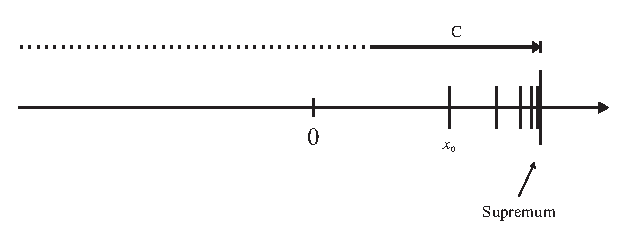
\includegraphics{skript/grafiken/supinfr1}
    \end{center}
    Sei $x_0$ die gr��te Zahl aus $\nat$, so dass $x_0, \ldots \in C$ existiert;  \\
    sei $x_1$ die gr��te Zahl aus $\{0 \ldots 9 \}$, so dass $x_0, x_1 \ldots \in C$ existiert; $\ldots$ \\
    sei $x_i$ die gr��te Zahl aus $\{0 \ldots 9 \}$, so dass $x_0, x_1 x_2 \ldots x_i \ldots \in C$ existiert. \par
    Man erh�lt einen unendlichen Dezimalzahl $x_0, x_1 x_2 \ldots$. \par
    Problem: F�r $C = \{ 0,9; \, 0,99; \, 0,999; \, \ldots \}$ w�re $0,\bar{9}$ nicht zul�ssig. \\
    L�sung: Endet $x_0,x_1 x_2 \ldots$ mit $\bar{9}$ ab der Stelle $i$, so ersetzen wir diese Folge durch $x_0,x_1 x_2 \ldots (x_{i-1}+1) \bar{0} \ldots$. \par
    $\Rightarrow$ Die so konstruierte Zahl ist das Supremum von $C$.
    \item Fall 2: $C$ ist von unten beschr�nkt, und alle Elemente aus $C$ sind positiv oder~$0$ (d.h. $C \subseteq \real^{\geq 0}$).
    \begin{center}
        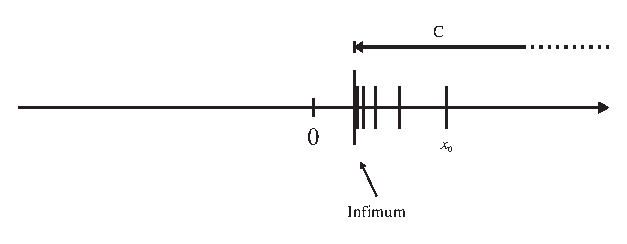
\includegraphics{skript/grafiken/supinfr2}
    \end{center}
    Sei $x_0$ die kleinste Zahl aus $\nat$, so dass $x_0,\ldots \in C$ existiert;  \\
    sei $x_1$ die kleinste Zahl aus $\{0 \ldots 9 \}$, so dass $x_0,x_1 \ldots \in C$ existiert; $\ldots$ \\
    sei $x_i$ die kleinste Zahl aus $\{0 \ldots 9 \}$, so dass $x_0,x_1 x_2 \ldots x_i \ldots \in C$ existiert. \par
    Man erh�lt einen unendlichen Dezimalzahl $x_0,x_1 x_2 \ldots$. \par
    $\Rightarrow$ Die so konstruierte Zahl ist das Infimum von $C$.
    \pagebreak

    \item Fall 3: $C$ ist von oben geschr�nkt, und alle Elemente aus $C$ sind negativ (d.h. $C \cap \real^{\geq 0} = \emptyset \Rightarrow C \subseteq \real^-$). \par
    \begin{center}
        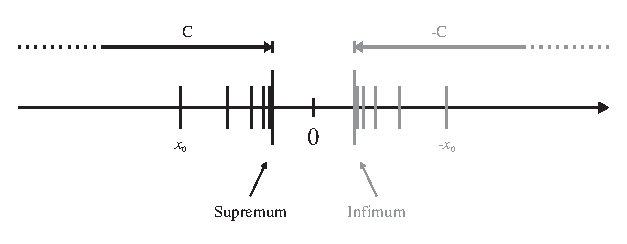
\includegraphics{skript/grafiken/supinfr3}
    \end{center}
    Man konstruiert $-C = \{ x \; | \; -x \in C \}$ und f�hrt es auf den Fall~2 zur�ck.
    $$\sup C = - \inf -C$$
    \item Fall 4: $C$ ist von unten geschr�nkt und $C \not\subseteq \real^{\geq 0} \Rightarrow C \cap \real^- \neq \emptyset$. \par
    \begin{center}
        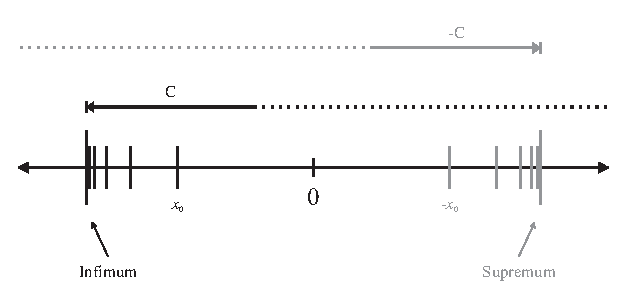
\includegraphics{skript/grafiken/supinfr4}
    \end{center}
    Man konstruiert $-C = \{ x \; | \; -x \in C \}$ und f�hrt es auf den Fall~1 zur�ck.
    $$\inf C = - \sup -C$$
\end{itemize}
\pagebreak

\textbf{Satz:\;} F�r jeden Schnitt $A, B$ von $\realpos$ gilt $\sup A = \inf B$. \par \abstand
\textbf{Beweis:\;} Alle $x \in B$ sind obere Schranke f�r $A$. Die kleinste obere Schranke (Supremum) von $A$ muss kleiner oder gleich $x$ f�r alle $x \in B$ sein. Das Supremum von $A$ ist untere Schranke von $B$. Damit ist die gr��te untere Schranke (Infimum) von $B$ gr��er oder gleich dem Supremum von $A$. \par
Das hei�t: $\sup A \leq \inf B$. Angenommen $\sup A < \inf B$ , dann g�be es ein $q \in \rat$, so dass $\sup A < q < \inf B$ wobei $q \notin A \wedge q \notin B$. Dies w�re ein Widerspruch, denn $A \cup B = \realpos$. \par
Damit ist $\sup A = \inf B$. \par \abstand
\textbf{Folgerung:\;} Jeder Schnitt von $\realpos$ ist ein Dedekind'scher Schnitt. Sei $A, B$ Schnitt in~$\realpos$ mit $c = \sup A = \inf B$.
\begin{itemize}
    \item Fall 1: $A$ hat ein gr��tes Element und $B$ hat \emph{kein} kleinstes Element.
    $$c \in A \wedge c \notin B \platz \Rightarrow \platz \sup A = \max A$$
    \item Fall 1: $A$ hat \emph{kein} gr��tes Element und $B$ hat ein kleinstes Element.
    $$c \notin A \wedge c \in B \platz \Rightarrow \platz \inf B = \min B$$
\end{itemize}

%%%%%%%%%%%%%%%%%%%%%%%%%%%%%%%%%%%%%%%%%%%%%%%%%%%%%%%%%%%%%%%%%%%%%%%%%%%%%%%
\subsection{Ungleichungen}
\textbf{Basisungleichungen:\;} F�r beliebige $a, b, c \in \real$ gilt:
\begin{itemize}
    \item $a \leq b \platz \Leftrightarrow \platz a+c \leq b+c$
    \item $a \leq b \platz \wedge \platz c \geq 0 \platz \Rightarrow \platz a \cdot c \leq b \cdot c$
    \item $0 \leq a \leq b \platz \Leftrightarrow \platz -b \leq -a \leq 0$
    \item $a > 0 \platz \Leftrightarrow \platz \frac{1}{a} > 0$
\end{itemize}

\textbf{Weitere Ungleichungen:\;} F�r beliebige $a, b, c, d \in \real$ gilt:
\begin{itemize}
    \item $a \leq b \platz \wedge \platz c\leq d \platz \Rightarrow \platz a+c \leq b+d$
    \item $a \leq b \platz \wedge \platz c \leq 0 \platz \Rightarrow \platz b \cdot c \leq a \cdot c$
    \item $0 \leq a \leq b \platz \wedge \platz 0 \leq c \leq d \platz \Rightarrow \platz 0 \leq a \cdot c \leq b \cdot d$
    \item $0 \leq a \leq b \platz \wedge \platz c \leq d \leq 0 \platz \Rightarrow \platz b \cdot c \leq a \cdot d \leq 0$
    \item $0 < a \leq b \platz \Rightarrow \platz 0 < \frac{1}{b} \leq \frac{1}{a}$
    \item $a \leq b < 0 \platz \Rightarrow \platz \frac{1}{b} \leq \frac{1}{a} < 0$
    \item $a^2 \geq 0$
\end{itemize}
\pagebreak

\textbf{Cauchy-Schwarz-Ungleichung:}\index{Cauchy-Schwarz-Ungleichung}
\begin{eqnarray*}
    \left( \sum_{i=1}^n a_i b_i \right)^2 &\leq& \sum_{i=1}^n a^2_i \cdot \sum_{i=1}^n b^2_i
\end{eqnarray*}

\textbf{Bernoulli-Ungleichung:}\index{Bernoulli-Ungleichung}
$$ (1+h)^n \geq 1 + nh \platz \platz \platz (\text{mit } h \geq -1, h \in \real, n \in \natpos) $$

Beweis �ber Induktion:
\begin{eqnarray}
    n=1 &\Rightarrow& 1+h \leq 1+h \nonumber \\
    n \rightarrow n+1 &\Rightarrow& (1+h)^{n+1} \nonumber \\
                                &=& (1+h)^n \cdot (1+h) \hspace{5cm} \eqname{Bemerkung: $1+h \geq 0$} \\
                                &\geq& (1+nh) \cdot (1+h) \eqname{nach Induktionsvoraussetzung} \\
                                &=& 1 + nh + h + nh^2 \nonumber \\
                                &=& 1+(n+1)h + n \cdot h^2 \nonumber \\
                                &\geq& 1+(n+1)h \nonumber
\end{eqnarray}

%%%%%%%%%%%%%%%%%%%%%%%%%%%%%%%%%%%%%%%%%%%%%%%%%%%%%%%%%%%%%%%%%%%%%%%%%%%%%%%
\subsection{Intervalle}
Die Klammern $[$ bzw. $]$ bezeichnen ein von links bzw. rechts abgeschlossenes Intervall; die Klammern $($ bzw. $)$ bezeichnen ein von links bzw. rechts offenes Intervall. Das hei�t f�r $a, b \in \real$ mit $a < b$:
\begin{eqnarray*}
    [a, b] &=& \{ x \in \real \; | \; a \leq x \leq b \} \\
    \left[ a, b \right) &=& \{ x \in \real \; | \; a \leq x < b \} \\
    \left( - \infty, b \right] &=& \{ x \in \real \; | \; x \leq b \} \\
    (a, \infty) &=& \{ x \in \real \; | \; a < x \} \\
    (- \infty, \infty) &=& \real \\
    (a-\varepsilon, a+\varepsilon) & & \text{$\varepsilon$-Umgebung von $a$ f�r $a \in \real$ und $\varepsilon > 0$}
\end{eqnarray*}
\pagebreak

%%%%%%%%%%%%%%%%%%%%%%%%%%%%%%%%%%%%%%%%%%%%%%%%%%%%%%%%%%%%%%%%%%%%%%%%%%%%%%%
\subsection{Betr�ge}
$$ | a | = \left\{
    \begin{array}{rcc}
        a & \text{falls} & a \geq 0 \\
        -a & \text{falls} & a < 0
    \end{array}
                      \right. $$

\textbf{Regeln:}
\begin{itemize}
    \item $- | a | \leq a \leq | a |$
    \item $| -a | = | a |$
    \item $| ab | = | a | \cdot | b |$
    \item $\left| \frac{a}{b} \right| = \frac{| a |}{| b |}$
    \item $| a | \leq b \platz \Leftrightarrow \platz -b \leq a \leq b$
    \item $- \left( | a | + | b | \right) \leq a + b \leq | a | + | b |$
    \item $\left| a+b \right| \leq \left| a \right| + \left| b \right|$ \hfill (Dreiecksungleichung)\index{Dreiecksungleichung}
    \item $\left| \overset{n}{\underset{i=1}{\sum}} \; a_i \right| \leq \overset{n}{\underset{i=1}{\sum}} \; | a_i |$
    \item $2 \cdot | a \cdot b | \leq a^2 + b^2$
\end{itemize}
Beweis:
\begin{eqnarray*}
    0 \leq (a-b)^2 &\wedge& 0 \leq (a+b)^2 \\
    0 \leq a^2 + b^2 - 2ab &\wedge& 0 \leq a^2 + b^2 + 2ab \\
    2ab \leq a^2 +  b^2 &\wedge& -(a^2+b^2) \leq 2ab \\
    -(a^2+b^2) \leq & 2ab & \leq a^2 + b^2 \\
    2 \cdot | a \cdot b | &\leq& a^2 + b^2
\end{eqnarray*}
\pagebreak

%%%%%%%%%%%%%%%%%%%%%%%%%%%%%%%%%%%%%%%%%%%%%%%%%%%%%%%%%%%%%%%%%%%%%%%%%%%%%%%
% Komplexe Zahlen
%%%%%%%%%%%%%%%%%%%%%%%%%%%%%%%%%%%%%%%%%%%%%%%%%%%%%%%%%%%%%%%%%%%%%%%%%%%%%%%
\section{Komplexe Zahlen}

%%%%%%%%%%%%%%%%%%%%%%%%%%%%%%%%%%%%%%%%%%%%%%%%%%%%%%%%%%%%%%%%%%%%%%%%%%%%%%%
\subsection{Einf�hrung}
\textbf{Idee:\;} Einf�hrung einer imagin�ren Einheit f�r $i = \sqrt{-1}$. Damit werden die folgenden Gleichungen l�sbar:
\begin{eqnarray*}
    x^2 + 1 &=& 0 \\
    x^2 &=& -1 \\
    x &=& \pm \sqrt{-1} \\
      &=& \pm i \\ \\
    x^2 -2x + 5 &=& 0 \\
    x_{1, 2} &=& 1 \pm \sqrt{-4} \\
            &=& 1 \pm \sqrt{4 (-1)} \\
            &=& 1 \pm 2 \sqrt{-1} \\
            &=& 1 \pm 2i
\end{eqnarray*}
\textbf{Definition:\;} Eine \emph{komplexe Zahl}\index{komplexe Zahlen} $z \in \comp$ hat die Form $z = x + yi$, wobei $x, y \in \real$ und $x = \text{Re } z$ der Realteil und $y = \text{Im } z$ der Imagin�rteil von $z$ genannt wird. \par \abstand
\textbf{Darstellung:\;} Eine komplexe Zahl wird als Paar $(x, y) \in \real^2$ bzw. als Punkt in der Ebene (komplexe Zahlenebene, \wichtig{Gauss-Ebene}) dargestellt. \par \abstand
\begin{center}
    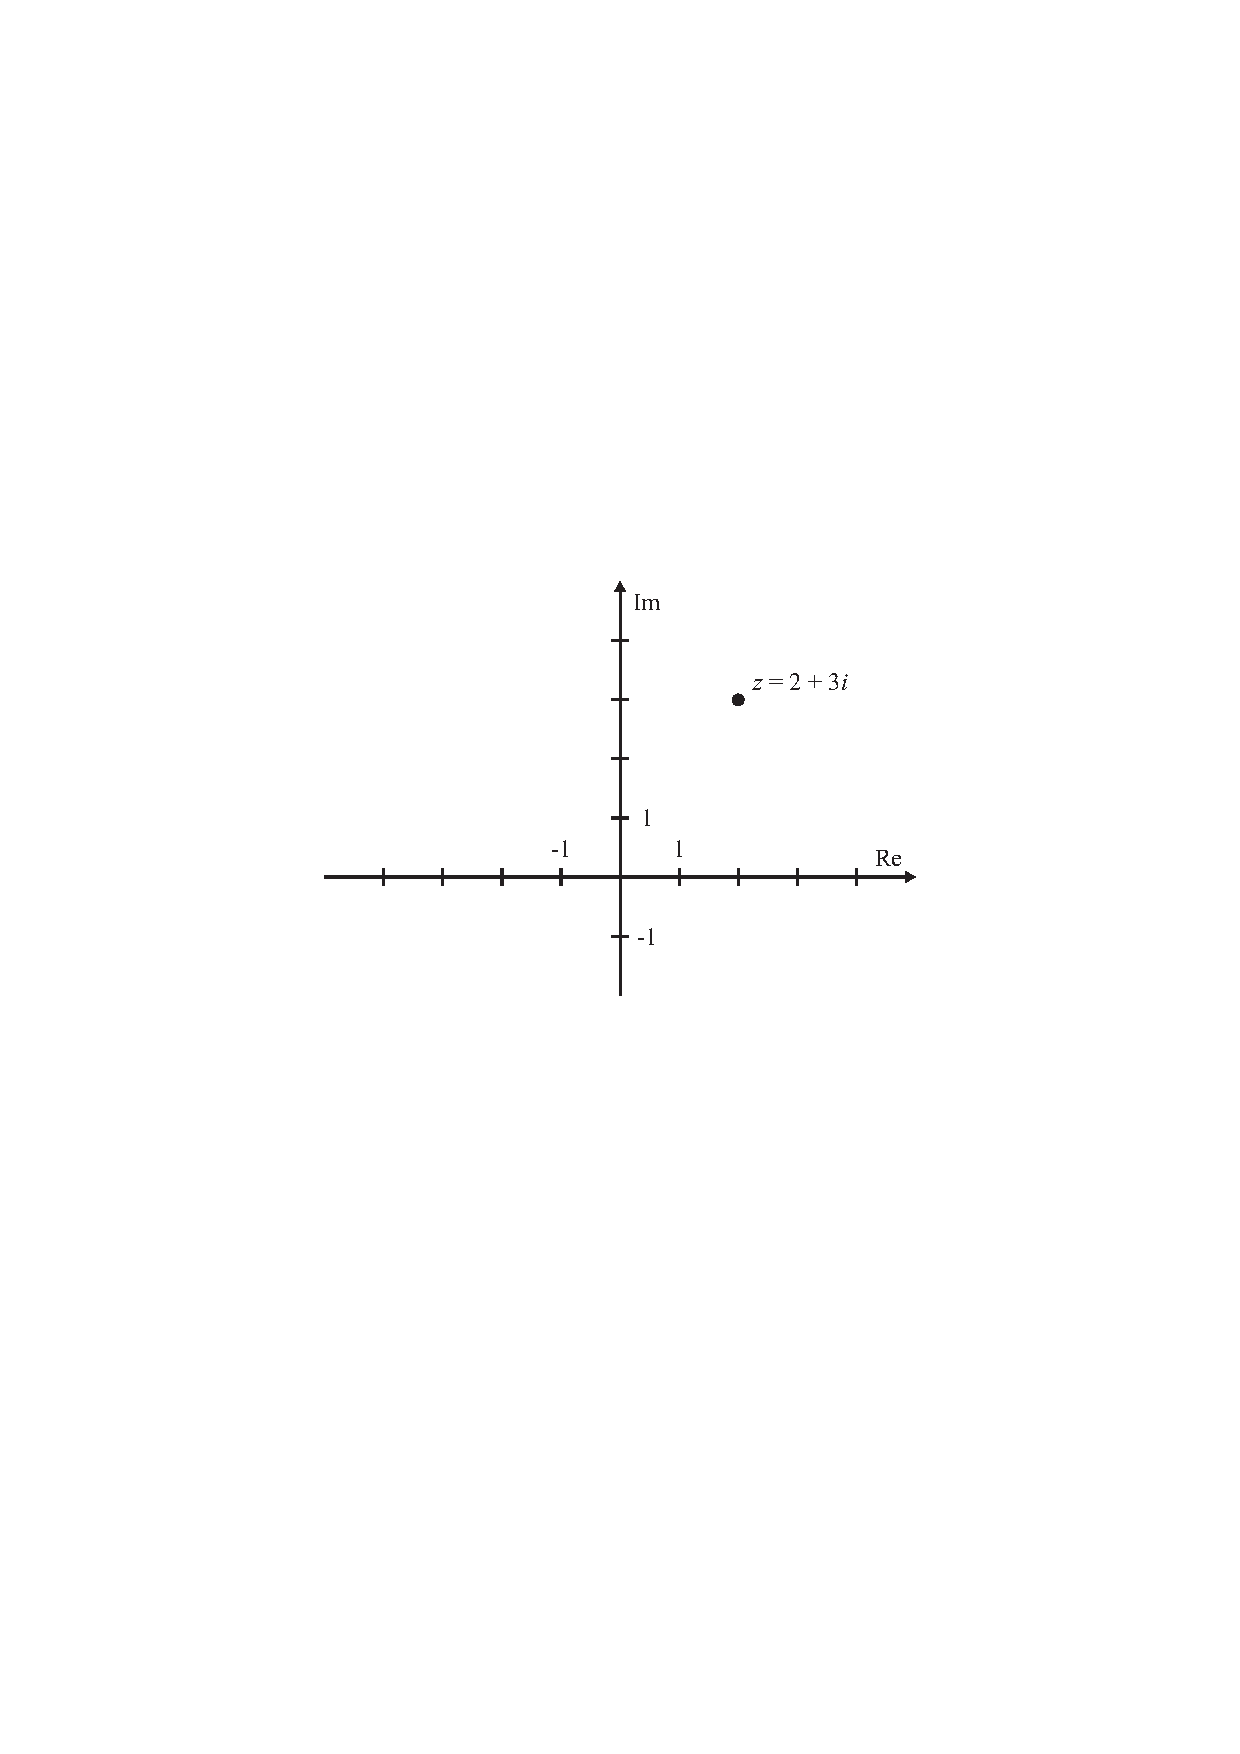
\includegraphics{skript/grafiken/komplexgauss}
\end{center}
Jede reelle Zahl $x \in \real$ ist auch eine komplexe Zahl $x + 0i$, insbesondere $0 = 0 + 0i $.

%%%%%%%%%%%%%%%%%%%%%%%%%%%%%%%%%%%%%%%%%%%%%%%%%%%%%%%%%%%%%%%%%%%%%%%%%%%%%%%
\subsection{Gleichheit und Rechenregeln}
\textbf{Rechenregeln:\;} $z = x + yi$ und $w = u + vi$ mit $z, w \in \comp$.
\begin{eqnarray*}
    z = w &\Leftrightarrow& x = u \; \wedge \; y = v \\
    z \pm w &=& (x \pm u) + (y \pm v) i \\
    z \cdot w &=& (xu - yv) + (xv + yu) i \\
    \frac{z}{w} &=& \frac{xu + yv}{u^2 + v^2} + \frac{yu - xv}{u^2 +  v^2} i \platz\platz \text{f�r $w \neq 0$} \\
\end{eqnarray*}
\textbf{Herleitung:\;} Multiplikation
\begin{eqnarray*}
    z \cdot w &=& (x+yi)(u+vi) \\
              &=& xu + xvi + yiu + yivi \platz\platz \text{(Bemerkung: $i^2 = -1$)} \\
              &=& (xu - yv)  + (xv + yu) i
\end{eqnarray*}
\textbf{Herleitung:\;} Division
\begin{eqnarray*}
    \frac{z}{w} &=& \frac{x+yi}{u+vi} \\
                &=& \frac{(x+yi)(u-vi)}{(u+vi)(u-vi)} \\
                &=& \frac{(xu+yv)+(yu-xv)i}{u^2-v^2 i^2} \\
                &=& \frac{xu+yv}{u^2+v^2}+\frac{yu-xv}{u^2+v^2}i \\
\end{eqnarray*}
\pagebreak

%%%%%%%%%%%%%%%%%%%%%%%%%%%%%%%%%%%%%%%%%%%%%%%%%%%%%%%%%%%%%%%%%%%%%%%%%%%%%%%
\subsection{Konjugiert komplexe Zahl und Betrag}
\textbf{Definition:\;} F�r eine komplexe Zahl $z = x+yi \in \comp$ wird die Zahl $\overline{z} = x-yi$ die zu $z$ \wichtig{konjugiert komplexe Zahl} genannt. \par \abstand
\textbf{Folgerung:\;} $z \cdot \overline{z} = x^2 + y^2$
\begin{center}
    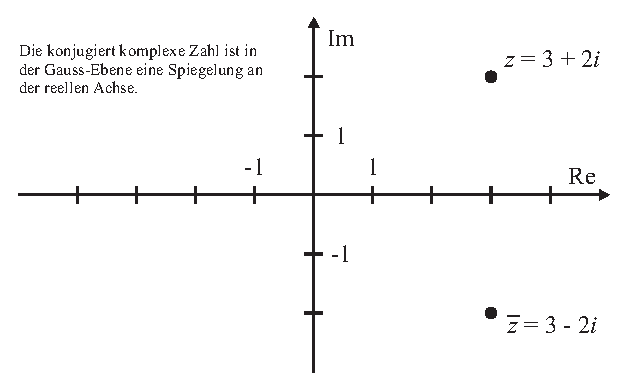
\includegraphics{skript/grafiken/komplexkonjugiert}
\end{center}
\seite

\textbf{Definition:\;} Der Betrag $|z| \in \real$ einer komplexen Zahl $z = x+yi$ ist definiert durch $|z| = \sqrt{x^2+y^2}$. \par \abstand
\textbf{Folgerung:\;} $|z| = \sqrt{z \cdot \overline{z}}$ \par \abstand
\textbf{Rechenregeln:\;} $z, w \in \comp$.
\begin{eqnarray*}
    \overline{z + w} &=& \overline{z} + \overline{w} \\
    \overline{z \cdot w} &=& \overline{z} \cdot \overline{w} \\
    \overline{\left( \frac{z}{w} \right)} &=& \frac{\overline{z}}{\overline{w}} \\
    \overline{\overline{z}} &=& z \\
    \text{Re } z &=& \frac{1}{2} (z + \overline{z}) \\
    \text{Im } z &=& \frac{1}{2i} (z - \overline{z}) \\
    | z \cdot w | &=& |z| \cdot |w| \\
    \left| \frac{z}{w} \right| &=& \frac{|z|}{|w|} \\
    | \overline{z} | &=& |z|
\end{eqnarray*}
\textbf{Herleitung:\;} $\overline{z \cdot w} = \overline{z} \cdot \overline{w}$ mit $z = x + yi$ und $w = u + vi$
\begin{eqnarray*}
    z \cdot w &=& (xu - yv) + (xv + yu)i \\
    \overline{z \cdot w} &=& (xu - yv) + (- xv - yu)i \\
    \overline{z} \cdot \overline{w} &=& (x-yi) \cdot (u-vi) \\
                                    &=& (xu - yv) + (- xv - yu)i
\end{eqnarray*}
\textbf{Herleitung:\;} $| z \cdot w | = |z| \cdot |w|$
\begin{eqnarray*}
    | z \cdot w | &=& \sqrt{(zw)(\overline{zw})} \\
                  &=& \sqrt{z \cdot w \cdot \overline{z} \cdot \overline{w}} \\
                  &=& \sqrt{z \cdot \overline{z} \cdot w \cdot \overline{w}} \\
                  &=& \sqrt{z \cdot \overline{z}} \cdot \sqrt{w \cdot \overline{w}} \\
                  &=& |z| \cdot |w|
\end{eqnarray*}

%%%%%%%%%%%%%%%%%%%%%%%%%%%%%%%%%%%%%%%%%%%%%%%%%%%%%%%%%%%%%%%%%%%%%%%%%%%%%%%
\subsection{Polarform}\index{Polarform}
\textbf{Definition:\;} Jede komplexe Zahl $z \in \comp$ ist eindeutig bestimmt durch ihre Polarkordinaten $|z|$ und $\arg z$, wobei das Argument (Phase) von $z$, der Winkel zwischen der positiven reellen Achse und dem Strahl von $0$ nach $z$ ist, der mit (entgegen) den Uhrzeigersinn negativ (positiv) gemessen wird. Der Hauptwert f�r $\arg z$ wird aus $(-\pi, \pi]$ gew�hlt. \par \abstand
\textbf{Achtung:\;} F�r die Zahl $0$ ist $\arg$ nicht definiert! \par \abstand
\textbf{Beispiel:\;} $z = 2 + 2i$ und $w = \sqrt{3} - i$
\begin{center}
    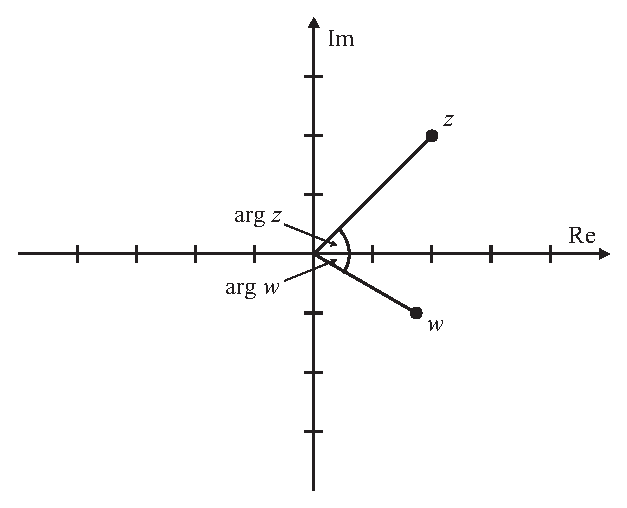
\includegraphics{skript/grafiken/komplexpolar}
\end{center}
$$ |z| = \sqrt{8} \platz\platz \arg z = \frac{\pi}{4} \platz\platz\platz\platz |w| = \sqrt{3+1} = 2 \platz\platz \arg w = - \frac{\pi}{6} $$
\pagebreak

\textbf{Kartische Darstellung $\mapsto$ Polardarstellung:}
$$ z = x+yi \platz \mapsto \platz |z|=\sqrt{x^2+y^2} \platz \arg = \left\{
    \begin{array}{rcc}
        \arccos \frac{x}{|z|} & \text{falls} & y \geq 0 \\
        - \arccos \frac{x}{|z|} & \text{falls} & y < 0
    \end{array}
                                                                   \right. $$
\textbf{Polardarstellung $\mapsto$ Kartische Darstellung:}
$$ r = |z| \platz \varphi = \arg z \platz \mapsto \platz z = r \cdot \cos \varphi + r \cdot i \cdot \sin \varphi $$

%%%%%%%%%%%%%%%%%%%%%%%%%%%%%%%%%%%%%%%%%%%%%%%%%%%%%%%%%%%%%%%%%%%%%%%%%%%%%%%
\subsection{Eulers komplexe Exponentialfunktion}

\textbf{Definition:\;} \wichtig{Eulers komplexe Exponentialfunktion}\index{komplexe Exponentialfunktion}\index{Exponentialfunktion, komplexe} ist definiert durch
$$ e^{i\varphi} = \cos \varphi + i \sin \varphi $$
Bemerkungen:
\begin{enumerate}
    \item In diesem Fall handelt es sich um eine Definition. Es ist jedoch auch die einzig sinnvolle Erweiterung der reellen Exponentialfunktion auf komplexe Zahlen.
    \item $\left| e^{i \varphi} \right| = \sqrt{\cos^2 \varphi + \sin^2 \varphi} = \sqrt{1} = 1$ \\
    D.h. $e^{i \varphi}$ liegt auf dem Einheitskreis.
    \item W�chst $\varphi(t) = \alpha + \omega t$ linear, so bewegt sich $z(t) = e^{i \varphi(t)}$ mit konstanter Winkelgeschwindigkeit auf dem Einheitskreis. \par
    Beispiel: $\alpha = \frac{\pi}{2}$ und $\omega = \frac{\pi}{12}$
    \begin{center}
        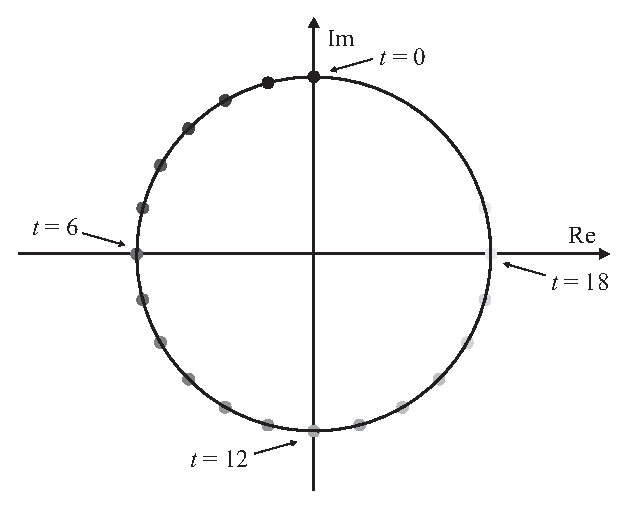
\includegraphics{skript/grafiken/komplexeuler}
    \end{center}
\end{enumerate}
\seite

\textbf{Exponentialform:\;} Man erweitert Eulers komplexe Exponentialfunktion auf alle komplexen Zahlen.
$$ e^{x+yi} = e^x \cdot e^{yi} $$
D.h. $ \left| e^{x+yi} \right| = e^x \platz \text{und} \platz \arg \left( e^{x+yi} \right) = y \pm 2k\pi \in \left( -\pi, \pi \right] $ \par \abstand \abstand

\textbf{Vorteile:\;} Einfache Multiplikations- und Divisionsformeln.
\begin{eqnarray*}
    z &=& |z| \cdot e^{i \varphi} \\
    w &=& |w| \cdot e^{i \psi} \\
    z \cdot w &=& |z| \cdot e^{i \varphi} \cdot |w| \cdot e^{i \psi} = |z| \cdot |w| \cdot e^{i \varphi} \cdot e^{i \psi} = |z| \cdot |w| \cdot e^{i \cdot \left( \varphi + \psi \right)} \\
    \frac{z}{w} &=& \frac{|z|}{|w|} \cdot \frac{e^{i \varphi}}{e^{i \psi}} = \frac{|z|}{|w|} \cdot e^{i \cdot \left( \varphi - \psi \right)}
\end{eqnarray*}

\textbf{Satz (De Moivre):}
\begin{enumerate}
    \willbuch
    \item $e^{i \varphi} \cdot e^{i \psi} = e^{i \left( \varphi + \psi \right)}$
    \begin{eqnarray*}
        e^{i \varphi} \cdot e^{i \psi} &=& \left( \cos \varphi + i \sin \varphi \right) \cdot \left( \cos \psi + i \sin \psi \right) \\
                                       &=& \cos \varphi \cdot \cos \psi - \sin \varphi \cdot \sin \psi + i \left( \sin \varphi \cdot \cos \psi + \cos \varphi \cdot \sin \psi \right) \\
                                       &=& \cos \left( \varphi + \psi \right) + i \sin \left( \varphi + \psi \right) \\
                                       &=& e^{i \left( \varphi + \psi \right) }
    \end{eqnarray*}
    \item $\left( e^{i \varphi} \right)^n = e^{i n \varphi}$ (Beweis �ber Induktion von a))
    \item $\overline{\left( e^{i \varphi} \right)} = e^{i \left( - \varphi \right)} = \frac{1}{e^{i \varphi}}$
    \begin{eqnarray*}
        \overline{\left( e^{i \varphi} \right)} &=& \overline{\left( \cos \varphi + i \sin \varphi \right)} \\
                                                &=& \cos \varphi - i \sin \varphi \\
                                                &=& \cos \varphi + i \left( - \sin \varphi \right) \\
                                                &=& \cos (- \varphi) + i \sin (- \varphi) \\
                                                &=& e^{i \left( - \varphi \right)} \\
                                                &=& \frac{1}{e^{i \varphi}}
    \end{eqnarray*}

\end{enumerate}
\pagebreak

\textbf{Einheitswurzel in $\comp$:} \par \abstand
\textbf{Definition:\;} $\sqrt[n]{1}$ bezeichnet in $\comp$ die Menge aller Nullstellen des Polynoms $x^n - 1$ (d.h. $\loes$ von $x^n = 1$).

$$\sqrt[n]{1} = \{ \zeta_0, \zeta_1, \zeta_2, \ldots \zeta_{n-1} \} = \left\{ 1, e^{i \cdot 1 \cdot \frac{2\pi}{n}}, e^{i \cdot 2 \cdot \frac{2\pi}{n}}, \ldots e^{i \cdot \left( n-1 \right) \cdot \frac{2\pi}{n}} \right\} $$

Bemerkung:\; In $\real$ ist es nur die positive Wurzel, falls sie existiert.
\begin{eqnarray*}
    \text{in $\real$} \platz \sqrt[2]{1} &=& 1 \\
    \text{in $\comp$} \platz \sqrt[2]{1} &=& \{ 1, -1 \}
\end{eqnarray*}

�berpr�fung der Formel durch Potenzieren:
$$\left( e^{i \cdot \left( j \cdot \frac{2\pi}{n} \right)} \right)^n = e^{i \cdot n \cdot j \cdot \frac{2\pi}{n}} = e^{i \cdot \left( 2\pi j \right) } = 1$$

\textbf{Wurzel beliebiger Zahlen in $\comp$:} \par \abstand
$\sqrt[n]{a}$ (mit $a = |a| \cdot e^{i \varphi}$) wird folgenderma�en bestimmt:
$$ \sqrt[n]{a} \Rightarrow \sqrt[n]{|a|} \cdot e^{i \cdot \frac{\varphi}{n}} $$
Dies ist das erste Element der L�sungsmenge. Alle weiteren L�sungen durch Multiplikation dieser L�sung mit den L�sungen der n-ten Einheitswurzel ermittelt.
$$ \sqrt[n]{a} = \left\{ \left. \sqrt[n]{|a|} \cdot e^{i \cdot \frac{\varphi}{n}} \cdot \zeta_j \; \right| \; 0 \leq j \leq n \right\} $$
�berpr�fung der Formel durch Potenzieren:
$$\left( \sqrt[n]{|a|} \cdot e^{i \cdot \frac{\varphi}{n}} \right)^n = \sqrt[n]{|a|}^n \cdot \left( e^{i \cdot \frac{\varphi}{n}} \right)^n = |a| \cdot e^{i \varphi} = a$$
\pagebreak

\textbf{Beispiel:\;} Zu bestimmen ist $\sqrt[3]{2 + 2i}$.
\begin{eqnarray*}
    a &=& 2 + 2i \\
    |a| &=& \sqrt{2^2 + 2^2} = \sqrt{8} \\
    \sqrt[3]{|a|} &=& \sqrt[3]{\sqrt{8}} = \sqrt{2} \\
    \arg a &=& \varphi = \frac{\pi}{4} \\
    \sqrt[3]{a} &\Rightarrow& \sqrt{2} \cdot e^{i \cdot \frac{\pi}{4} \cdot \frac{1}{3}} = \sqrt{2} \cdot e^{i \cdot \frac{\pi}{12}} \\
    \sqrt[3]{a} &=& \left\{ \sqrt{2} \cdot e^{i \cdot \frac{\pi}{12}}, \sqrt{2} \cdot e^{i \cdot \left( \frac{\pi}{12} + \frac{2\pi}{3} \right) }, \sqrt{2} \cdot e^{i \cdot \left( \frac{\pi}{12} + \frac{4\pi}{3} \right) } \right\} \\
                &=& \left\{ \sqrt{2} \cdot e^{i \cdot \frac{\pi}{12}}, \sqrt{2} \cdot e^{i \cdot \frac{3\pi}{4} }, \sqrt{2} \cdot e^{i \cdot \frac{17\pi}{12} } \right\}
\end{eqnarray*}
\begin{center}
    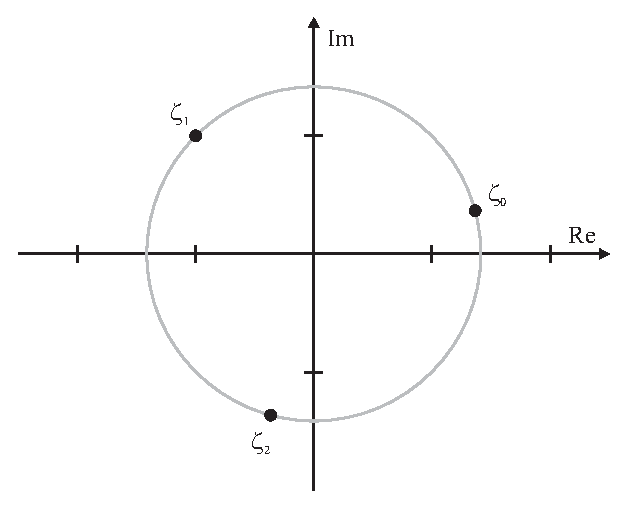
\includegraphics{skript/grafiken/komplexwurzel}
\end{center}

%%%%%%%%%%%%%%%%%%%%%%%%%%%%%%%%%%%%%%%%%%%%%%%%%%%%%%%%%%%%%%%%%%%%%%%%%%%%%%%
\subsection{Fundamentalsatz der Algebra (Gauss)}
\textbf{Satz:\;} Jedes komplexe Polynom $p(z) = a_n z^n + a_{n-a} z^{n-1} + \ldots + a_1 z + a_0$ mit $a_i \in \comp$ hat eine komplexe Nullstelle. Folglich kann $p(z)$ in der Form
$$ a_n \cdot \prod_{\mu=1}^n (z-z_{\mu}) $$
dargestellt werden, wobei $z_{\mu}$ die Nullstellen von $p(z)$ sind.
\pagebreak

%%%%%%%%%%%%%%%%%%%%%%%%%%%%%%%%%%%%%%%%%%%%%%%%%%%%%%%%%%%%%%%%%%%%%%%%%%%%%%%
\subsection{Harmonische Schwingungen}
\textbf{Definition:\;} Eine physikalische Gr��e $s(t) = A \cdot \cos(\omega t + \alpha)$ mit $A, \omega, \alpha \in \real$ wird harmonische Schwingung genannt.
\begin{itemize}
    \item Amplitude: $A$
    \item Periode: $\frac{2\pi}{\omega}$
    \item Frequenz: $\frac{\omega}{2\pi}$
\end{itemize}

\textbf{�berlagerung:\;} Wir betrachten �berlagerung von zwei harmonischen Schwingungen gleicher Frequenz.
\begin{center}
    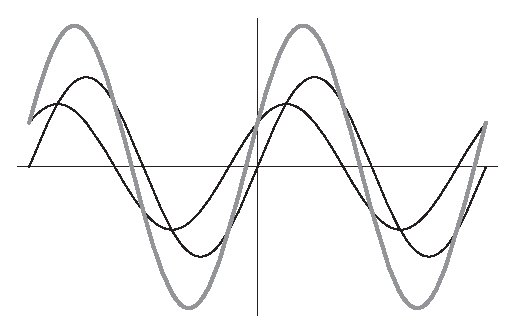
\includegraphics{skript/grafiken/harmonischeschwingungen}
\end{center}
\begin{eqnarray*}
    s_1(t) &=& A_1 \cdot \cos (\omega t + \alpha_1) \\
    s_2(t) &=& A_2 \cdot \cos (\omega t + \alpha_2) \\
    s(t) &=& s_1(t) + s_2(t)
\end{eqnarray*}
$s_i(t)$ wird behandelt als Realteil von $A_j \cdot e^{\omega t + \alpha_j}$:
\begin{eqnarray*}
    s_1(t) + s_2(t) &=& \text{Re} (A_1 \cdot e^{i (\omega t + \alpha_1)} + A_2 \cdot e^{i (\omega t + \alpha_2)}) \\
                    &=& \text{Re} (A_1 \cdot e^{i \omega t} \cdot e^{i \alpha_1} + A_2 \cdot e^{i \omega t} \cdot e^{i \alpha_2} \\
                    &=& \text{Re} ((A_1 \cdot e^{i \alpha_1} + A_2 \cdot e^{i \alpha_2}) \cdot e^{i \omega t} \\
                    &=& \text{Re} ((a_1 + a_2) \cdot e^{i \omega t}) \\
                    &=& \text{Re} (A \cdot e^{i \varphi} \cdot e^{i \omega t}) \\
                    &=& \text{Re} (A \cdot e^{i (\omega t + \varphi)}) \\
                    &=& A \cdot \cos (\omega t + \varphi)
\end{eqnarray*}
Damit handelt es sich um eine harmonische Schwingung (wobei $A = |a_1 + a_2|$ und $\varphi = \arg (a_1 + a_2)$).
\pagebreak

\textbf{Wechselstromnetze:\;} Wir betrachten die Wechselspannung~$u(t)$ mit dem Strom~$j(t)$.
\begin{eqnarray*}
    u(t) &=& u_0 \cos (\omega t + \alpha) \\
    j(t) &=& j_0 \cos (\omega t + \beta)
\end{eqnarray*}
\begin{itemize}
    \item $u(t)$ ist Realteil von $U(t) = u_0 \cdot e^{i(\omega t + \alpha)}$
    \item $j(t)$ ist Realteil von $J(t) = j_0 \cdot e^{i (\omega t + \beta)}$
    \item komplexer Widerstand: $Z(t) = \frac{U(t)}{J(t)}$ ist eine Konstante
    $$Z(t) = \frac{U(t)}{J(t)} = \frac{u_0 \cdot e^{i \cdot (\omega t + \alpha)}}{j_0 \cdot e^{i \cdot (\omega t + \beta)}} = \frac{u_0 \cdot e^{i \omega t} \cdot e^{i \alpha}}{j_0 \cdot e^{i \omega t} \cdot e^{i \beta}} = \frac{u_0}{j_0} \cdot e^{i (\alpha - \beta)} \in \comp $$
    \item $\text{Re }Z$: Wirkwiderstand
    \item $\text{Im }Z$: Blindwiderstand
    \item $|Z|$: Scheinwiderstand
\end{itemize} \abstand \abstand

Symbole:
\begin{itemize}
    \item Ohmscher Widerstand: $Z = R$
    \begin{center}
        \includegraphics{skript/grafiken/widerstaendeohm}
    \end{center}
    \item Kapazit�t $C$ \par
    kapazitiver Widerstand: $Z = \frac{1}{i \omega C}$
    \begin{center}
        \includegraphics{skript/grafiken/widerstaendekap}
    \end{center}
    \item Induktivit�t $L$ \par
    induktiver Widerstand: $Z = i \omega L$
    \begin{center}
        \includegraphics{skript/grafiken/widerstaendeind}
    \end{center}
\end{itemize}
\pagebreak

Beispiel:
\begin{center}
    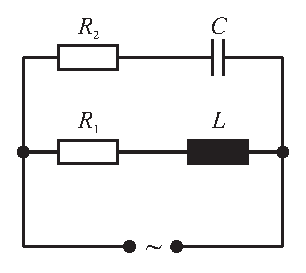
\includegraphics{skript/grafiken/widerstaendeschaltung}
\end{center}
Bei welcher Frequenz verh�lt sich der Gesamtwiderstand wie ein Ohmscher?
\begin{eqnarray*}
    Z &=& \frac{(R_1 + i \omega L)(R_2 + \frac{1}{i \omega C})}{R_1 + i \omega L + R_2 + \frac{1}{i \omega C}} \\
      &=& \frac{R^2_1 R_2 + R_1 R^2_2 + R_1 \frac{1}{\omega^2 C^2} + R_2 L^2 \omega + i (R^2_2 \omega L - \frac{R^2}{\omega C} + \frac{L}{\omega C^2} - \frac{\omega L^2}{C})}{(R_1 + R_2)^2 + (\omega L - \frac{1}{\omega C})^2}
\end{eqnarray*}
Suche $\omega$, so dass $\text{Im }Z = 0$ wird.
\begin{eqnarray*}
    \omega \left( R^2_2 L - \frac{L^2}{C} \right) &=& \frac{1}{\omega} \left( \frac{R^2_1}{C} - \frac{L}{C^2} \right) \\
    \omega &=& \sqrt{\frac{\frac{R^2_1}{C} - \frac{L}{C^2}}{R^2_2 L - \frac{L^2}{C}}}
\end{eqnarray*}

\chapter{Grenzwerte von Folgen und Funktionen}

%%%%%%%%%%%%%%%%%%%%%%%%%%%%%%%%%%%%%%%%%%%%%%%%%%%%%%%%%%%%%%%%%%%%%%%%%%%%%%%
% Grenzwerte von Folgen
%%%%%%%%%%%%%%%%%%%%%%%%%%%%%%%%%%%%%%%%%%%%%%%%%%%%%%%%%%%%%%%%%%%%%%%%%%%%%%%
\section{Grenzwerte von Folgen}
%%%%%%%%%%%%%%%%%%%%%%%%%%%%%%%%%%%%%%%%%%%%%%%%%%%%%%%%%%%%%%%%%%%%%%%%%%%%%%%
\subsection{Einleitung}
\textbf{Definition:\;} Eine Folge ist eine Funktion  von $\nat$ (oder $\natpos$) nach $\real$, d.h. jedem $n \in \nat$ wird ein $a_n \in \real$ zugeordnet. \par \abstand
\textbf{Schreibweisen:\;} $(a_n)_{n \in \nat}$, $(a_n)_{n \geq 0}$ oder $a_0, a_1, a_2, \ldots$ \par \abstand
\textbf{Beispiele:}
\begin{itemize}
    \item explizite Definition:
    \begin{enumerate}
        \item konstante Folge ($c \in \real$):
        \begin{itemize}
            \item $a_n = c$
            \item $(c)_{n \in \nat}$
        \end{itemize}
        \item arithmetische Folge ($c, d \in \real$):
        \begin{itemize}
            \item $a_n = c + n \cdot d$
            \item $(c + n \cdot d)_{n \in \nat}$
            \item $c, c+d, c+2d, \ldots$
        \end{itemize}
        \item geometrische Folge ($c, q \in \real, q \neq 0$):
        \begin{itemize}
            \item $a_n = c \cdot q^n$
            \item $(c \cdot q^n)_{n \in \nat}$
            \item $c, cq, cq^2, cq^3, \ldots$
        \end{itemize}
        \seite
        \item harmonische Folge ($n \geq 1$):
        \begin{itemize}
            \item $a_n = \frac{1}{n}$
            \item $\left( \frac{1}{n} \right)_{n \in \natpos}$
            \item $1, \frac{1}{2}, \frac{1}{3}, \ldots$
        \end{itemize}
    \end{enumerate}
    \seite
    \item rekursive Definition:
    \begin{enumerate}
        \item konstante Folge:
        \begin{itemize}
            \item $a_0 = c$, $a_{n+1} = a_n$
        \end{itemize}
        \item arithmetische Folge:
        \begin{itemize}
            \item $a_0 = c$, $a_{n+1} = a_n + d$
        \end{itemize}
        \item geometrische Folge:
        \begin{itemize}
            \item $a_0 = c$, $a_{n+1} = a_n \cdot q$
        \end{itemize}
        \item Fibonacci-Zahlen:
        \begin{itemize}
            \item $a_0 = 0$, $a_1 = 1$, $a_{n+2} = a_n + a_{n+1}$
        \end{itemize}
    \end{enumerate}
\end{itemize}

%%%%%%%%%%%%%%%%%%%%%%%%%%%%%%%%%%%%%%%%%%%%%%%%%%%%%%%%%%%%%%%%%%%%%%%%%%%%%%%
\subsection{Beschr�nktheit und Monotonie}\index{Beschr�nktheit}\index{Monotonie}
\textbf{Definition:\;} Die Folge $(a_n)_{n \in \nat}$ hei�t genau dann $\ldots$, wenn
\begin{itemize}
    \item beschr�nkt
    \begin{eqnarray*}
        \exists K \in \real \platz \forall n \in \nat \platz |a_n| \leq K
    \end{eqnarray*}
    \item von unten beschr�nkt
    \begin{eqnarray*}
        \exists K \in \real \platz \forall n \in \nat \platz a_n \geq K
    \end{eqnarray*}
    \item von oben beschr�nkt
    \begin{eqnarray*}
        \exists K \in \real \platz \forall n \in \nat \platz a_n \leq K
    \end{eqnarray*}
    \item monoton wachsend
    \begin{eqnarray*}
        \forall n \in \nat \platz a_{n+1} \geq a_n
    \end{eqnarray*}
    \item streng monoton wachsend
    \begin{eqnarray*}
        \forall n \in \nat \platz a_{n+1} > a_n
    \end{eqnarray*}
    \item monoton fallend
    \begin{eqnarray*}
        \forall n \in \nat \platz a_{n+1} \leq a_n
    \end{eqnarray*}
    \item streng monoton fallend
    \begin{eqnarray*}
        \forall n \in \nat \platz a_{n+1} < a_n
    \end{eqnarray*}
\end{itemize} \abstand \abstand

%%%%%%%%%%%%%%%%%%%%%%%%%%%%%%%%%%%%%%%%%%%%%%%%%%%%%%%%%%%%%%%%%%%%%%%%%%%%%%%
\subsection{Konvergenz}\index{Konvergenz}
\textbf{Definition:\;} Eine Folge $(a_n)_{n \in \nat}$ konvergiert (strebt) gegen den \emph{Grenzwert}\index{Grenzwert (Folgen)} $a$, falls
$$\forall \varepsilon > 0 \platz \exists n_0 \in \nat \platz \forall n \geq n_0 \platz |a_n - a| < \varepsilon$$
Schreibweise:
\begin{eqnarray*}
    a_n \underset{n \to \infty}{\longrightarrow} a &\text{oder}& a_n \longrightarrow a \\
    \lim_{n \to \infty} a_n = a &\text{oder}& \lim a_n = a
\end{eqnarray*} \abstand

\textbf{Satz:\;} F�r jede konvergente Folge $(a_n)_{n \in \nat}$ gilt die Eindeutigkeit des Grenzwerts.
$$ \lim_{n \to \infty} a_n = a \platz \wedge \platz \lim_{n \to \infty} a_n = b \platz \Rightarrow \platz a = b $$
\textbf{Beweis:}
\begin{eqnarray*}
    \varepsilon &:=& \frac{|b-a|}{3} \\
    \exists n_{0, a} \platz \forall n \geq n_{0, a} & & |a_n - a| < \varepsilon \\
    \exists n_{0, b} \platz \forall n \geq n_{0, b} & & |a_n - b| < \varepsilon \\
    n_0 &=& \max (n_{0, a}, n_{0, b}) \\
    n &>& n_0 \\
    | a_n - a | < \varepsilon &\wedge& | a_n - b | < \varepsilon \\
    | a - b | &\leq& | a - a_n | + | a_n - b | \\
              &<& \varepsilon + \varepsilon \\
              &\leq& 2 \varepsilon \\
              &\leq& \frac{2}{3} \cdot | a - b | \\
    \frac{1}{3} \cdot | a - b | &<& 0 \platz \text{Widerspruch!} \\
    \Rightarrow \platz a &=& b
\end{eqnarray*}

\textbf{Satz:\;} Jede konvergente Folge ist beschr�nkt. \par \abstand
\textbf{Beweis:}
$$ \varepsilon := 1 \platz \Rightarrow \platz  \exists n_0 \platz \forall n \geq n_0 | a - a_n | \leq 1$$
Man w�hlt:
$$ K  = \max \{ |a_0|, |a_1|, \ldots |a_{n_0}-1|, |a-1|, |a+1| \} $$
Dann ist:
$$ |a_n| \leq K \platz \forall n \in \nat $$
\pagebreak

%%%%%%%%%%%%%%%%%%%%%%%%%%%%%%%%%%%%%%%%%%%%%%%%%%%%%%%%%%%%%%%%%%%%%%%%%%%%%%%
\subsection{Nullfolgen und Teilfolgen}
\textbf{Definition:\;} Eine Folge, die gegen 0 konvergiert, wird \wichtig{Nullfolge} genannt. \par \abstand

\textbf{Definition:\;} Ist $(a_n)_{n \in \nat}$ eine Folge und $0 \leq n_0 < n_1 < n_2 < \ldots$ eine Folge von nat�rlichen Zahlen, dann wird $(a_{n_i})_{i \in \nat} = a_{n_0}, a_{n_1}, a_{n_2}, \ldots$ eine \wichtig{Teilfolge} von $(a_n)_{n \in \nat}$ genannt. \par \abstand

\textbf{Satz:\;} Wenn $(a_n)_{n \in \nat}$ gegen $a$ konvergiert, dann konvergiert jede Teilfolge von $(a_n)_{n \in \nat}$ gegen $a$. \par \abstand

\textbf{Beispiele:}
\begin{enumerate}
    \item Zu zeigen: $a_n = \frac{1}{n}$ ist eine Nullfolge.
    \begin{itemize}
        \item $\varepsilon$ ist gr��er $0$.
        \item Man sucht eine Zahl $n_0$, so dass f�r $n \geq n_0$ gilt: $|a_n - 0| < \varepsilon$.
        \item Man wei�, damit ist $\frac{1}{n} < \varepsilon$.
        \item Daraus folgt, dass $0 < \frac{1}{n} < \varepsilon$ genau dann, wenn $n > \frac{1}{\varepsilon}$.
        \item Deswegen setzt man $n_0 := \left\lceil \frac{1}{\varepsilon} \right\rceil$.
        \item F�r alle $n \geq n_0$ gilt dann $n \geq n_0 > \left\lceil \frac{1}{\varepsilon} \right\rceil \geq \frac{1}{\varepsilon}$.
        \item Daraus folgt: $\frac{1}{n} < \varepsilon$.
        \item Damit ist $a_n = \frac{1}{n}$ eine Nullfolge: $\underset{n \to \infty}{\lim} \frac{1}{n} = 0 $.
    \end{itemize}
    \item Zu zeigen: $b_n = \frac{1}{n^2 + 4n + 5}$ ist eine Nullfolge
    \begin{itemize}
        \item $c_n = (n^2 + 4n + 5)_{n \in \nat}$ bildet nur auf Zahlen in $\nat$ ab.
        \item $c_n$ ist streng monoton wachsend.
        \item Damit ist $b_n$ streng monoton fallend.
        \item Daraus folgt: $b_n$ ist eine Teilfolge von $a_n = \frac{1}{n}$.
        \item Damit ist auch $b_n$ eine Nullfolge: $\underset{n \to \infty}{\lim} \frac{1}{n^2 + 4n + 5} = 0 $.
    \end{itemize}
\end{enumerate}
\pagebreak

%%%%%%%%%%%%%%%%%%%%%%%%%%%%%%%%%%%%%%%%%%%%%%%%%%%%%%%%%%%%%%%%%%%%%%%%%%%%%%%
\subsection{Partialsummenfolge}
\textbf{Definition:\;} F�r eine Folge $(a_n)_{n \in \nat}$ sei $(s_n)_{n \in \nat}$ folgenderma�en definiert:
$$ s_n = \sum_{i = 0}^n a_i $$
Man nennt $(s_n)_{n \in \nat}$ die \wichtig{Partialsummenfolge} von $(a_n)_{n \in \nat}$ oder die zu $(a_n)_{n \in \nat}$ geh�rende \wichtig{Reihe}. \par \abstand
Konvergiert $(s_n)_{n \in \nat}$ gegen $S$, dann schreibt man
$$ \sum_{n = 0}^{\infty} a_n =  \lim_{n \to \infty} s_n = S $$

%%%%%%%%%%%%%%%%%%%%%%%%%%%%%%%%%%%%%%%%%%%%%%%%%%%%%%%%%%%%%%%%%%%%%%%%%%%%%%%
\subsection{Bestimmte Divergenz}\index{Divergenz, bestimmt}
\textbf{Definition:\;} Die Folge $(a_n)_{n \in \nat}$ divergiert gegen den \emph{uneigentlichen Grenzwert}\index{Grenzwert, uneigentlicher (Folgen)}~$\pm \infty$ (bestimmte Divergenz), falls
$$ \forall K \in \real \platz \exists n_0 \platz \forall n \geq n_0 \platz a_0 \gtrless K $$

\textbf{Beispiele:}
\begin{enumerate}
    \item[1.] $a_n = c \cdot q^n$
\end{enumerate}
\vspace{-0.4cm}
\begin{align*}
    \lim_{n \to \infty} a_n &= \left\{ \begin{array}{r@{\platz\text{falls}\platz}ccr@{\platz}c@{\platz}ccc}
      \text{unbestimmt divergent} & q & \leq & -1 & \text{und} & c & \neq & 0 \\
      0 & |q| & < & 1 & \text{oder} & c & = & 0 \\
      c & q & = & 1 & \text{und} & c & \neq & 0 \\
      \infty & q & > & 1 & \text{und} & c & \neq & 0
    \end{array} \right. \\
    \intertext{ \begin{enumerate}
        \item[2.] $a_n = c + n \cdot d$
    \end{enumerate} }
    \lim_{n \to \infty} a_n &= \left\{ \begin{array}{r@{\platz\text{falls}\platz}ccc}
      c & d & = & 0 \\
      \infty & d & > & 0 \\
      -\infty & d & < & 0
    \end{array} \right.
\end{align*}
\pagebreak

%%%%%%%%%%%%%%%%%%%%%%%%%%%%%%%%%%%%%%%%%%%%%%%%%%%%%%%%%%%%%%%%%%%%%%%%%%%%%%%
\subsection{Grenzwertregeln}
\textbf{Satz:\;} Seien $(a_n)_{n \in \nat}$ und $(b_n)_{n \in \nat}$ kovergente Folgen mit $\underset{n \to \infty}{\lim} a_n = a$ und $\underset{n \to \infty}{\lim} b_n =~b$, dann gilt:
\begin{itemize}
    \item $\underset{n \to \infty}{\lim} (a_n + b_n) = a + b$
    \item $\underset{n \to \infty}{\lim} (a_n \cdot b_n) = a \cdot b$ \hfill (Spezialfall: $\underset{n \to \infty}{\lim} (c \cdot b_n) = c \cdot b$)
    \item $\underset{n \to \infty}{\lim} \left( \frac{a_n}{b_n} \right) = \frac{a}{b}$ \hfill (falls $b \neq 0$ und $b_n \neq 0$ f�r $n > n_0$)
    \item $\underset{n \to \infty}{\lim} |a_n| = |a|$
    \item $\underset{n \to \infty}{\lim} \sqrt{|a_n|} = \sqrt{|a|} $
\end{itemize}
\abstand

\textbf{Beweis:\;} Zu zeigen: $a + b$ ist Grenzwert von $(a_n + b_n)_{n \in \nat}$.
$$ (a_n + b_n)_{n \in \nat} \platz \Leftrightarrow \platz \forall \varepsilon > 0 \platz \exists n_0 \platz \forall n > n_0 \platz |a_n + b_n - (a + b)| < \varepsilon $$
Sei $\varepsilon > 0$, dann w�hlt man $\varepsilon' = \frac{\varepsilon}{2} > 0$ und $n \geq n_0$.
\begin{eqnarray*}
    & \exists n_{0, a} \platz \forall n \geq n_{0, a} \platz |a_n - a| < \varepsilon' \\
    & \exists n_{0, b} \platz \forall n \geq n_{0, b} \platz |b_n - b| < \varepsilon' \\
    & n_0 = \max (n_{0, a}, n_{0, b})
\end{eqnarray*}
\begin{eqnarray*}
    |a_n + b_n - (a + b)| &=& | a_n - a + b_n -b | \\
                          &\leq& | a_n - a | + | b_n - b | \\
                          &<& \varepsilon' + \varepsilon' = \varepsilon
\end{eqnarray*}

\textbf{Beweis:\;} Zu zeigen: $a \cdot b$ ist Grenzwert von $(a_n \cdot b_n)_{n \in \nat}$
\begin{eqnarray*}
    | a_n \cdot b_n - a \cdot b | &=& | a_n \cdot b_n  \underbrace{ - a_n \cdot b + a_n \cdot b }_{0} - a \cdot b | \\
                                  &\leq& | a_n | \cdot | b_n - b | + | b | \cdot | a_n - a | \\
                                  &<& \frac{\varepsilon}{2} +  \frac{\varepsilon}{2} = \varepsilon \\ \\
    \begin{array}{r} \varepsilon' \\ \\ \varepsilon'' \end{array} &
    \begin{array}{c} = \\ \\ = \end{array} &
    \left. \begin{array}{c} \frac{\varepsilon}{2 \cdot (|a| + 1)} \\ \\ \frac{\varepsilon}{2 \cdot (|b| + 1)} \end{array} \right\} \text{ f�r } n > \max(n_{0, b}, n_{0, a})
\end{eqnarray*}
\pagebreak

\textbf{Beispiele:}
\begin{eqnarray*}
    \underset{n \to \infty}{\lim} \left( \frac{2n+3}{n+1} \right) &=& \underset{n \to \infty}{\lim} \left( \frac{n \cdot \left( 2 + \frac{3}{n} \right) }{ n \cdot \left( 1 + \frac{1}{n} \right) } \right) \\
                                                                  &=& \frac{ \underset{n \to \infty}{\lim} \left( 2 + \frac{3}{n} \right) }{ \underset{n \to \infty}{\lim} \left( 1 + \frac{1}{n} \right) } \\
                                                                  &=& \frac{ \underset{n \to \infty}{\lim} 2 + \underset{n \to \infty}{\lim} 3 \cdot \underset{n \to \infty}{\lim} \left( \frac{1}{n} \right) }{ \underset{n \to \infty}{\lim} 1 + \underset{n \to \infty}{\lim} \left( \frac{1}{n} \right) } \\
                                                                  &=& \frac{2 + 3 \cdot 0}{1 + 0} = 2 \\ \\ \\
    \underset{n \to \infty}{\lim} \sqrt{ \frac{8n^3 + 5n -18}{36n^3-100n^2} } &=& \sqrt{\underset{n \to \infty}{\lim} \left( \frac{n^3 \cdot \left( 8 + \frac{5}{n^2} - \frac{18}{n^3} \right) }{ n^3 \cdot \left( 36 - 100 \cdot \frac{1}{n} \right) } \right) } \\
                                                                              &=& \sqrt{\frac{\underset{n \to \infty}{\lim} \left( 8 + \frac{5}{n^2} - \frac{18}{n^3} \right) }{ \underset{n \to \infty}{\lim} \left( 36 - 100 \cdot \frac{1}{n} \right) } } \\
                                                                              &=& \sqrt{\frac{2}{9}} \\
                                                                              &=& \frac{\sqrt{2}}{3}
\end{eqnarray*}
\pagebreak

%%%%%%%%%%%%%%%%%%%%%%%%%%%%%%%%%%%%%%%%%%%%%%%%%%%%%%%%%%%%%%%%%%%%%%%%%%%%%%%
\subsection{Vergleichskriterium}\index{Vergleichskriterium}
\textbf{Satz:\;} Seien $(a_n)_{n \in \nat}, (b_n)_{n \in \nat}, (c_n)_{n \in \nat}$ Folgen mit $a_n \leq b_n \leq c_n$ f�r $n \geq n_0$ und ist $\underset{n \to \infty}{\lim} a_n = \underset{n \to \infty}{\lim} c_n = c$, dann ist auch $\underset{n \to \infty}{\lim} b_n = c$ (wobei $c \in \real \cup \{ \pm \infty \}$). \par \abstand

\textbf{Beispiele:}
\begin{itemize}
    \item Zu bestimmen ist der Grenzwert von $a_n = \frac{\sin^2 n}{n}$.
    \begin{itemize}
        \item Da $\sin^2 n \leq 1$, ist $0 \leq \frac{\sin^2 n}{n} \leq \frac{1}{n}$.
        \item Au�erdem ist $\underset{n \to \infty}{\lim} 0 = \underset{n \to \infty}{\lim} \left( \frac{1}{n} \right) = 0$.
        \item Daraus folgt: $\underset{n \to \infty}{\lim} \left( \frac{\sin^2 n}{n} \right) = 0$.
    \end{itemize}
    \item Zu zeigen: Der Grenzwert von $a_n = \sqrt[n]{n}$ mit $n \geq 1$ ist $1$.
    \begin{itemize}
        \item Sei $b_n = \sqrt[n]{n} - 1$ mit $n \geq 1$.
        \item Die Folge $b_n$ ist von unten durch $0$ begrenzt.
        \begin{eqnarray*}
            (b_n + 1)^n &=& \left( \sqrt[n]{n} -1 + 1 \right)^n = n \\
            n &=& (1 + b_n)^n = 1 + \begin{pmatrix} n \\ 1 \end{pmatrix} \cdot b_n + \begin{pmatrix} n \\ 2 \end{pmatrix} \cdot b_n^2 + \ldots \\
            n &\geq& 1 + \begin{pmatrix} n \\ 2 \end{pmatrix} \cdot b_n^2 = 1 + \frac{n(n-1)}{2} \cdot b_n^2 \\
            (n - 1) &\geq& \frac{n(n-1)}{2} \cdot b_n^2 \\ \\
            1 &\geq& \frac{n}{2} \cdot b_n^2 \\ \\
            b_n^2 &\leq& \frac{2}{n} \\
        \end{eqnarray*}
        \item Da $b_n^2$ von unten auch durch $0$ begrenzt und von oben durch $\frac{2}{n}$, und die Grenzwerte beide $0$ sind, ist nach dem Vergleichskriterium auch der Grenzwert von $b_n^2$ $0$.
        \item Der Grenzwert von $b_n$ ist damit auch $0$.
        \item Da $a_n = b_n + 1$, ist auch $\lim a_n = \lim b_n + 1 = 1$.
    \end{itemize}
\end{itemize}

\textbf{Folgerung:\;} Die Limesbildung erh�lt schwache Ungleichungen, d.h. sind $(a_n)_{n \in \nat}$ und $(b_n)_{n \in \nat}$ konvergent und $a_n \leq b_n$ (f�r $n \geq n_0$), dann $\underset{n \to \infty}{\lim} a_n \leq \underset{n \to \infty}{\lim} b_n$. \par \abstand
Achtung: Dies gilt \emph{nicht} f�r starke Ungleichungen.
\pagebreak

%%%%%%%%%%%%%%%%%%%%%%%%%%%%%%%%%%%%%%%%%%%%%%%%%%%%%%%%%%%%%%%%%%%%%%%%%%%%%%%
\subsection{Monotoniekriterium}\index{Monotoniekriterium}
\textbf{Satz:\;} Jede monoton wachsende (fallende), beschr�nkte Folge $(a_n)_{n \in \nat}$ ist konvergent. \par \abstand
\textbf{Beweis:}
\begin{itemize}
    \item Ist $(a_n)_{n \in \nat}$ monoton wachsend, dann ist $a = \sup \{ a_n \; | \; n \in \nat \}$ Grenzwert.
    \item Ist $(a_n)_{n \in \nat}$ monoton fallend, dann ist $a = \inf \{ a_n \; | \; n \in \nat \}$ Grenzwert.
\end{itemize}

\textbf{Beispiel:}
\begin{itemize}
    \item Geometrische Reihe (ohne Monotoniekriterium):
    \begin{eqnarray}
        a_n &=& c \cdot q^n \eqname{geometrische Folge} \\
        s_n &=& \sum_{k=0}^n c \cdot q^n = c \cdot \frac{1-q^{n+1}}{1-q} \hspace{4cm} \eqname{geometrische Reihe} \\
        \sum_{k=0}^{\infty} a_n &=& \lim_{n \to \infty} s_n \nonumber \\
                                &=& \lim_{n \to \infty} \left( c \cdot \frac{1-q^{n+1}}{1-q} \right) \nonumber \\ \nonumber \\
                                &=& c \cdot \frac{1 - \lim_{n \to \infty} q^{n+1}}{1-q} \nonumber \\ \nonumber \\
                                &=& \left\{ \begin{array}{r@{\platz\text{falls}\platz}rcr}
                                  \text{divergent} & q & \leq & -1 \\
                                  \frac{c}{1-q} & |q| & < & 1 \\
                                  c & q & = & 1 \\
                                  \infty & q & > & 1
                                \end{array} \right. \nonumber
    \end{eqnarray}
    \pagebreak

    \item Reihe von $\left( \frac{1}{n^2} \right)_{n \in \nat}$:
    \begin{itemize}
        \item Bildung der Reihe:
        \begin{eqnarray*}
            s_n &=& 1 + \frac{1}{2^2} + \frac{1}{3^2} + \ldots + \frac{1}{n^2} \\
                &=& \sum_{k=1}^n \frac{1}{k^2}
        \end{eqnarray*}
        \item Monotonie:
        \begin{eqnarray*}
            s_{n+1} - s_n &=& \sum_{k=1}^{n+1} \frac{1}{k^2} - \sum_{k=1}^n \frac{1}{k^2} \\
                        &=& \frac{1}{(n+1)^2} \geq 0 \\ \\
                        &\Rightarrow& s_{n+1} \geq s_n
        \end{eqnarray*}
        Damit ist $s_n$ monoton wachsend. \abstand
        \item Beschr�nktheit:\; Zu zeigen: $0 \leq a_n \leq 2$
        \begin{eqnarray}
            \frac{1}{n^2} &\leq& \frac{1}{n(n-1)} \nonumber \\
                        &=& \frac{n-n+1}{n(n-1)} \nonumber  \\
                        &=& \frac{1}{n-1}-\frac{1}{n} \nonumber \\ \nonumber \\ \nonumber \\
            s_n &\leq& 1 + \left( \frac{1}{1} - \frac{1}{2} \right) + \left( \frac{1}{2} - \frac{1}{3} \right) + \left( \frac{1}{3} - \frac{1}{4} \right) + \ldots + \left( \frac{1}{n-1} - \frac{1}{n} \right) \nonumber \\
                &=& 2 - \frac{1}{n} \eqname{Teleskopsumme} \\
                &<& 2 \nonumber
        \end{eqnarray}
        Damit ist $s_n$ von oben durch 2 beschr�nkt. \abstand
        \item Daraus folgt: $s_n$ ist konvergent. \abstand
        \item Man kann zeigen:
        $$ \lim_{n \to \infty} s_n = \frac{\pi^2}{6} $$
    \end{itemize}
    \pagebreak

    \item Reihe von $\left( \frac{1}{k!} \right)_{n \in \nat}$:
    \begin{itemize}
        \item Bildung der Reihe:
        \begin{eqnarray*}
            s_n &=& \sum_{k=0}^n \frac{1}{k!} \\
                &=& 1 + 1 + \frac{1}{2} + \frac{1}{3!} + \ldots + \frac{1}{n!}
        \end{eqnarray*}
        \item Monotonie:
        \begin{eqnarray*}
            s_{n+1} - s_n &=& \frac{1}{(n+1)!} \geq 0 \\ \\
                          &\Rightarrow& s_{n+1} \geq s_n
        \end{eqnarray*}
        Damit ist $s_n$ monoton wachsend.
        \item Beschr�nktheit:\; Zu zeigen: $0 \leq a_n \leq 3$
        \begin{eqnarray*}
            \frac{1}{n!} &\leq& \frac{1}{1 \cdot 2 \cdot 3 \cdot \ldots \cdot n} \leq \frac{1}{2^{n-1}} \\ \\ \\
            s_n &\leq& 1 + \sum_{k=1}^n \frac{1}{2^{k-1}} \\
                &=& 1 + \sum_{k=0}^{n-1} \left( \frac{1}{2} \right)^k \\
                &=& 1 + \frac{1-\left(\frac{1}{2}\right)^n}{1-\frac{1}{2}} \\
                &<& 1 + \frac{1}{\frac{1}{2}} \leq 3
        \end{eqnarray*}
        Damit ist $s_n$ von oben durch 3 beschr�nkt. \abstand
    \end{itemize}
    \textbf{Definition:\;} Die Euler'sche Zahl $e$ ist definiert als
    $$ e := \lim_{n \to \infty} \left( \sum_{k=0}^n \frac{1}{k!} \right)$$
    \pagebreak

    \item Folge $c_n = \left( 1 + \frac{1}{n} \right)^n$
    \begin{itemize}
        \item Anwenundung:\; $c_n$ ist der Faktor der Verwertung eines Kapitals in einem Jahr bei Zinssatz von $100\%$ und $n$-maliger Aufzinsung.
        \begin{center}\begin{tabular}{lll}
            $n=1$ & j�hrliche Aufzinsung & $c_1 = 2$ \\
            $n=12$ & monatliches Aufzinsung & $c_{12} = 2,613$ \\
            $n=365$ & t�gliche Aufzinsung & $c_{365} = 2,714$
        \end{tabular}\end{center}
        Beoachtung:\; $c_n$ n�hert sich mit steigendem $n$ dem Wert von $e$. \par \abstand
        Ziel:\; Nachweis f�r $\underset{n \to \infty}{\lim} c_n = e$ \abstand
        \item Monotonie:
        \begin{align*}
            \frac{c_n}{c_{n-1}} &= \frac{\left( 1 + \frac{1}{n} \right)^n}{\left( 1 + \frac{1}{n-1} \right)^{n-1}} \\
                                &= \frac{\left( n+1 \right)^n \cdot \left( n-1 \right)^{n-1} \cdot \left( n-1 \right) \cdot n }{ n^n \cdot n^{n-1 \cdot \left( n-1 \right) \cdot n } } \\
                                &= \frac{n}{n-1} \cdot \frac{ \left( n+1 \right)^n \cdot \left( n-1 \right)^n }{ n^{2n} } \\
                                &= \frac{n}{n-1} \cdot \left( \frac{n^2-1}{n^2} \right)^n  \\
                                &= \frac{n}{n-1} \cdot \left( 1 - \frac{1}{n^2} \right)^n \\
                                \intertext{ Anwendung der Bernoulli-Ungleichung: $ (1-a)^n \geq 1 - n \cdot a \platz \text{mit} \platz a = \frac{1}{n^2} $ }
                                &\geq \frac{n}{n-1} \cdot \left( 1 - \frac{1}{n} \right) \\
                                &= 1
        \end{align*}
        Damit ist $c_n$ monoton wachsend.
        \pagebreak

        \item Beschr�nkung:\; Zu zeigen: $c_n \leq e$ f�r alle $n \in \nat$.
        \begin{eqnarray*}
            c_n &=& \left( 1+\frac{1}{n} \right)^n \\
                &=& \sum_{k=0}^n \left( {n \atop k} \right) \cdot \left( \frac{1}{n} \right)^k \\
                &\overset{*}{\leq}& \sum_{k=0}^n \frac{1}{k!} \\
                &\leq& e \\ \\
            \overset{*}{\Rightarrow} \platz \left( {n \atop k} \right) \cdot \left( \frac{1}{n} \right)^k &=& \frac{n \cdot (n-1) \cdot \ldots \cdot (n-k+1)}{k! \cdot n \cdot n \cdot \ldots \cdot n} \\
                                                                                                          &\leq& \frac{1}{k!}
        \end{eqnarray*}

        \item Behauptung:\; $\underset{n \to \infty}{\lim} c_n = e$ \par \abstand
        $N \geq 1$ beliebig, aber fest ($n > N$):
        \begin{eqnarray*}
            c_n &=& \left( 1 + \frac{1}{n} \right)^n \\
                &=& \sum_{k=0}^n \left( { n \atop k } \right) \cdot \left( \frac{1}{n^k} \right) \\
                &\geq& \sum_{k=0}^N \left( {n \atop k} \right) \cdot \left( \frac{1}{n^k} \right) \\
                &=& \sum_{k=0}^N \frac{1}{k!} \cdot 1 \cdot \left( 1 - \frac{1}{n} \right) \cdot \left( 1 - \frac{2}{n} \right) \cdot \ldots \cdot \left( 1 - \frac{k-1}{n} \right) \\
                &\geq& \sum_{k=0}^N \frac{1}{k!} \cdot \left( 1 - \frac{N}{n} \right)^N
        \end{eqnarray*}
        \pagebreak

        \begin{eqnarray*}
            \lim_{n \to \infty} c_n &\geq& \lim_{n \to \infty} \left( \sum_{k=0}^N \frac{1}{k!} \cdot \left( 1-\frac{N}{n} \right) \right) \\
                                            &=& \sum_{k=0}^n \frac{1}{k!} \left( \lim_{n \to \infty} \left( 1 - \frac{N}{n} \right) \right)^N \\
                                            &=& \sum_{k=0}^N \frac{1}{k!}
        \end{eqnarray*}
        Vergleichskriterium:
        \begin{eqnarray*}
            e & \geq & \lim_{n \to \infty} c_n \geq \sum_{k=0}^N \frac{1}{k!} \\
            e & \geq & \lim_{n \to \infty} c_n \geq \lim_{N \to \infty} \left( \sum_{k=0}^N \frac{1}{k!} \right) \geq e
        \end{eqnarray*}
        Daraus folgt: $\underset{n \to \infty}{\lim} c_n = e$.
    \end{itemize}
\end{itemize}
\pagebreak

%%%%%%%%%%%%%%%%%%%%%%%%%%%%%%%%%%%%%%%%%%%%%%%%%%%%%%%%%%%%%%%%%%%%%%%%%%%%%%%
\subsection{Exponentialfunktion als Grenzwert}
\textbf{Satz:\;} F�r jedes $x \in \real$ existiert der Grenzwert
$$ \exp(x) := \lim_{n \to \infty} \left( 1+\frac{x}{n} \right)^n $$

\begin{itemize}
    \item Monotonie:\; wie f�r $\left( 1+\frac{1}{n} \right)^n$ \abstand
    \item Beschr�nkheit:\; Man betrachtet zwei F�lle.
    \begin{enumerate}
        \item Fall:\; $x \leq 0$ f�r alle $n > -x$
        \begin{eqnarray*}
            0 &\leq& 1 + \frac{x}{n} \\
              &\leq& 1 \\ \\
            \Rightarrow \platz 0 &\leq& \left( 1+\frac{x}{n} \right)^n
        \end{eqnarray*}
        \item Fall:\; $x>0$
        \begin{eqnarray*}
            a_n &:=& \left( 1+\frac{x}{n} \right)^n \\
            b_n &:=& \left( 1+\frac{-x}{n} \right)^n \hspace{1cm} \text{(1. Fall: $b_n$ ist konvergent)} \\
            a_n b_n &=& \left( 1+\frac{x}{n} \right)^n \cdot \left( 1-\frac{x}{n} \right)^n \\
                    &=& \left( 1-\frac{x^2}{n^2} \right)^n \\
                    &=& \left( 1- \frac{\frac{x^2}{n}}{n} \right)^n \\
                    &\geq& 1-\frac{x^2}{n} \nonumber \\ \\
            \Rightarrow \platz a_n b_n &\leq& 1 \hspace{1cm} (n \geq x^2)
        \end{eqnarray*}
    \end{enumerate}
    \pagebreak

    \item Vergleichskriterium:
    \begin{eqnarray*}
        \underset{n \to \infty}{\lim} a_n b_n &=& 1 \\ \\
        a_n &=& \frac{a_n b_n}{b_n} \\ \\
        \underset{n \to \infty}{\lim} a_n &=& \frac{\underset{n \to \infty}{\lim} a_n b_n}{\underset{n \to \infty}{\lim} b_n} \\ \\
                                        &=& \frac{1}{\underset{n \to \infty}{\lim} b_n}
    \end{eqnarray*}

    \item Mit �hnlichen Argumenten kann man zeigen:
    \begin{itemize}
        \item Produkt zweier Exponentialfunktionen:
        $$ \exp(x+y) = \exp(x) \cdot \exp(y) $$
        \item Euler'sche Zahl:
        $$ \exp(1) = \lim_{n \to \infty} \left( 1+\frac{1}{n} \right)^n = e $$
        \item f�r $x \in \nat$:
        $$ \exp(x) = e^x $$
        \item auch f�r $x \in \ganz$, d.h. f�r $x = -n$:
        $$ \exp(x) = \exp(-n) = \frac{1}{e^n} $$
        \item f�r $q = \frac{m}{n}$ mit $m \in \ganz$, $n \in \natpos$
        $$ \exp \left( \frac{m}{n} \right) = \left( \sqrt[n]{e} \right)^m = e^{\frac{m}{n}} $$
    \end{itemize}
\end{itemize}
\pagebreak

%%%%%%%%%%%%%%%%%%%%%%%%%%%%%%%%%%%%%%%%%%%%%%%%%%%%%%%%%%%%%%%%%%%%%%%%%%%%%%%
\subsection{Cauchy-Kriterium}\index{Cauchy-Kriterium}
\textbf{Satz:\;} Eine Folge $(a_n)_{n \in \nat}$ ist genau dann konvergent, wenn
$$ \forall \varepsilon > 0 \platz \exists n_0 \in \nat \platz \forall n,m \geq n_0 \platz |a_n - a_m| < \varepsilon $$

\textbf{Anwendung:\;}
\begin{itemize}
    \item Die harmonische Reihe $s_n$ ist \emph{nicht} kovergent.
    \begin{eqnarray*}
        s_n &=& \sum_{k=1}^n \frac{1}{k} \\
            &=& \underbrace{\frac{1}{1}} + \underbrace{\frac{1}{2}} + \underbrace{\frac{1}{3} + \frac{1}{4}} + \underbrace{\frac{1}{5} + \ldots + \frac{1}{8}} + \underbrace{\frac{1}{9} + \ldots + \frac{1}{16}} + \ldots + \frac{1}{n} \\
            &\geq& 1 + \frac{1}{2} + \underbrace{\frac{1}{4} + \frac{1}{4}} + \underbrace{\frac{1}{8} + \frac{1}{8} + \frac{1}{8} + \frac{1}{8}} + \underbrace{8 \cdot \frac{1}{16}} + \ldots + \frac{1}{n} \\
            &\geq& 1 + \underbrace{\frac{1}{2} + \frac{1}{2} + \frac{1}{2} + \frac{1}{2} + \ldots + \frac{1}{2}}_{\left\lfloor \log_2 n \right\rfloor} \\
            &=& 1 + \frac{1}{2} \left\lfloor \log_2n \right\rfloor
    \end{eqnarray*}
    Das hei�t, $s_n$ ist nicht beschr�nkt.
    \item Die alteriende harmonische Reihe $s_n$ ist konvergent.
    $$ s_n = \sum_{k=1}^n \frac{(-1)^{k+1}}{k} = 1 - \frac{1}{2} + \frac{1}{3} - \frac{1}{4} + \ldots + \frac{(-1)^{n+1}}{n} $$
    Sei $\varepsilon > 0$ und $n_0 := \left\lceil \frac{1}{\varepsilon} \right\rceil$ mit $n, m \geq n_0$ und ohne Beschr�nkung der Allgemeinheit $m > n$.
    \begin{eqnarray*}
        |a_m - a_n| &=& \left| \frac{(-1)^{n+2}}{n+1} + \frac{(-1)^{n+3}}{n+2} + \ldots + \frac{(-1)^{m+1}}{m} \right| \\ \\
                    &\leq& \frac{1}{n+1} \\ \\
                    &<& \varepsilon
    \end{eqnarray*}
\end{itemize}
\pagebreak

%%%%%%%%%%%%%%%%%%%%%%%%%%%%%%%%%%%%%%%%%%%%%%%%%%%%%%%%%%%%%%%%%%%%%%%%%%%%%%%
% Polynome und rationale Funktionen
%%%%%%%%%%%%%%%%%%%%%%%%%%%%%%%%%%%%%%%%%%%%%%%%%%%%%%%%%%%%%%%%%%%%%%%%%%%%%%%
\section{Polynome und rationale Funktionen}
%%%%%%%%%%%%%%%%%%%%%%%%%%%%%%%%%%%%%%%%%%%%%%%%%%%%%%%%%%%%%%%%%%%%%%%%%%%%%%%
\subsection{Polynome}
\textbf{Definition:\;} Ein \wichtig{Polynom} �ber einen kommutativen Ring $R$ ist ein formaler Ausdruck der Form
$$ \sum_{k=0}^n a_k x^k $$
wobei $a_k \in R$ und $a_n \neq 0$. Der Rang dieses Polynoms ist $n$. \par \abstand
Jedes Polynom bestimmt eine Funktion $R \rightarrow R$ durch Einsetzen von Werten f�r~$x$. \par \abstand
Die Polynome
$$ p(x) = \sum_{k=1}^n a_k x^k \platz \text{und} \platz q(x) = \sum_{k=1}^m b_k x^k $$
sind (syntaktisch) gleich (als formaler Ausdr�cke), falls $n=m$ und $a_k=b_k$ f�r $k=0, \ldots n$ \par \abstand

\textbf{Satz:\;} F�r Polynome �ber $\real$ (und �ber $\rat$ und $\comp$) gilt: $p(x)$ und $q(x)$ sind syntaktisch gleich, wenn die zugeh�rigen Polynomfunktion semanisch gleich sind.

%%%%%%%%%%%%%%%%%%%%%%%%%%%%%%%%%%%%%%%%%%%%%%%%%%%%%%%%%%%%%%%%%%%%%%%%%%%%%%%
\subsection{Horner-Schema}
Funktionswertbestimmung durch das \wichtig{Horner-Schema}:
\begin{eqnarray}
    f(x) &=& \sum_{k=0}^n a_k x^k \eqname{$2n$ Multiplikationen und $n$ Additionen} \\ \nonumber \\
         &=& a_n x^k + a_{n-1} x^{n-1} + \ldots + a_2 x^2 + a_1 x + a_0 \nonumber \\
         &=& \underbrace{ \underbrace{(\underbrace{(\underbrace{(\underbrace{(\underbrace{a_n}_{c_n} x + a_{n-1})}_{c_{n-1}} \cdot x \ldots a_3)}_{c_3} \cdot x + a_2)}_{c_2} \cdot x + a_1)}_{c_1} \cdot x + a_0}_{c_0} \nonumber \\
         & & \eqname{$n$ Multiplikationen und $n$ Additionen}
\end{eqnarray}

\textbf{Allgemeiner L�sungsweg:}
$$ \begin{array}{r|c|c|c|cc|c|c}
  f(x) =  & a_n & a_{n-1} & a_{n-1} & \multicolumn{2}{|c|}{\ldots} & a_1 & a_0 \\ \hline
    &     &             &                 & & &             & \\
  + &     & c_n \cdot x & c_{n-1} \cdot x & & & c_2 \cdot x & c_1 \cdot x \\ \hline
    & c_n & c_{n-1} & c_{n-2} & & c_2 & c_1 & c_0
\end{array} $$
Der Wert von $c_0$ ist der Funktionswert von $f(x)$. \par \abstand

\textbf{Beispiel:\;} Bestimme $f(3)$ von $f(x) = 2x^4 - 4x^3 + 3x + 10$.
$$ \begin{array}{r|r|r|r|r|r}
  f(3) =  & 2 & -4 & 0 & 3 & 10 \\ \hline
    &     &   &   &    & \\
  + &     & 6 & 6 & 18 & 63 \\ \hline
    & 2 & 2 & 6 & 21 & 73
\end{array} $$
Damit ist $f(3) = 73$. \par \abstand \abstand \abstand

\textbf{Satz:\;} Sei $f(x)$ das Polynom
$$ f(x) = \sum_{k=0}^n a_k x^k $$
mit $a_n \neq 0$, $n \geq 1$, $x_0 \in \real$, dann gilt:
$$ \begin{array}{rcl}
  c_n &=& a_n \\
  c_{n-1} &=& c_n \cdot b + a_{n-1} \\
  &\vdots& \\
  c_0 &=& c_1 \cdot b + a_0 \\ \\
  c_0 &=& f(x) \\ \\
  f(x_0) &=& (x-x_0) \cdot (c_n x^{n-1} + \ldots + c_2 x + c_1) + c_0
\end{array} $$
Koeffizientenvergleich bei $f(x_0)$ und $(x-x_0) \cdot (c_n x^{n-1} + \ldots + c_2 x + c_1) + c_0$ f�r~$x^k$
\begin{itemize}
    \item links: $a_k$
    \item rechts: $a_n - b \cdot c_{k+1} = b \cdot c_{k+1} + a_k - b \cdot c_{k+1} = a_k$.
\end{itemize}
\pagebreak

%%%%%%%%%%%%%%%%%%%%%%%%%%%%%%%%%%%%%%%%%%%%%%%%%%%%%%%%%%%%%%%%%%%%%%%%%%%%%%%
\subsection{Nullstellen}
\textbf{Definition:\;} $x_0 \in \real$ ist Nullstelle von $f(x)$, falls $f(x_0)=0$. \par \abstand
\textbf{Satz:\;} Ist $x_0$ Nullstelle von $f(x)$, dann existiert ein Polynom $g(x)$:
$$ f(x) = (x-x_0) \cdot g(x) $$
\textbf{Beweis:\;} folgt aus der Anwendung des Horner-Schemas. \par \abstand
\textbf{Definition:\;} $x_0$ ist $k$-fache Nullstelle des Polynoms $f(x)$, falls ein Polynom $g(x)$ existiert:
$$ f(x) = (x-x_0)^k \cdot g(x) $$

\textbf{Satz:\;} Jedes reele Polynom $f(x)$ kann folgenderma�en zerlegt werden:
$$ \sum_{k=0}^n a_k x^k = a_n \cdot \prod_{i=1}^l (x - b_i)^{k_i} \cdot \prod_{i=1}^m (x^2 + c_i x + d_i) $$
\begin{itemize}
    \item $k_1 + k_2 + \ldots + k_l + 2m = n$ ist Grad des Polynoms.
    \item $b_1, b_2, \ldots b_l$ sind $k_1, k_2, \ldots, k_l$-fache reelen Nullstellen von $f(x)$.
    \item Die Polynome $x^2 + c_i \cdot x + d_i$ haben keine reelen Nullstellen.
\end{itemize}

%%%%%%%%%%%%%%%%%%%%%%%%%%%%%%%%%%%%%%%%%%%%%%%%%%%%%%%%%%%%%%%%%%%%%%%%%%%%%%%
\subsection{Rationale Funktionen}\index{rationale Funktion}\index{Funktion, rationale}
\textbf{Definitionen:}
\begin{itemize}
    \item Eine \wichtig{ganz rationale Funktion} ist ein Poylnom.
    \item Eine \emph{(gebrochen) rationale Funktion}\index{gebrochen rationale Funktion} ist ein Quotient aus zwei Polynomen~$\frac{f(x)}{g(x)}$.
    \item Eine \wichtig{echt gebrochen rationale Funktion} ist ein Quotient von zwei Polynomen~$\frac{f(x)}{g(x)}$ mit $\text{Grad}(f(x))$ $<$ $\text{Grad}(g(x))$.
\end{itemize}

\textbf{Satz:\;} Jede rationale Funktion $\frac{p(x)}{q(x)}$ mit $\text{Grad}(p(x)) \geq \text{Grad}(q(x))$ l�sst sich darstellen in der Form
$$ \frac{p(x)}{q(x)} = h(x) + \frac{r(x)}{q(x)} $$
wobei $h(x)$ ganz rational und $\frac{r(x)}{q(x)}$ echt gebrochen rational ist.
\pagebreak

\textbf{Beweis:} \par \abstand
Bemerkung: Dieser Beweis zeigt, warum \wichtig{Polynomdivision} �berhaupt funktioniert. \par \abstand
Es seien die Polynome $p(x)$ und $q(x)$ gegeben:
\begin{eqnarray*}
    p(x) &=& \sum_{k=0}^n a_k x^k \\
    q(x) &=& \sum_{k=0}^m b_k x^k \platz \platz \platz \text{(mit $n \geq m$)}
\end{eqnarray*}
\begin{itemize}
    \item Induktion nach $d = n-m$
    \item Induktionsanfang: $d=0$, d.h. $n=m$ \par
    $$ p_1(x) = p(x) - \frac{a_n}{b_n} \cdot q(x) $$
    Behauptung: $\text{Grad}(p_1(x)) < n$ \par
    Koeffizient von $x^n$: $a_n - \frac{a_n}{b_n} \cdot b_n = 0$
    $$ \frac{p(x)}{q(x)} = \frac{a_n}{b_n} \cdot \frac{q(x)}{q(x)} + \frac{p_1(x)}{q(x)} $$
    Damit ist $p_1(x) = r(x)$ und $\frac{a_n}{b_n} = h(x)$ aus dem Satz.
    \item Induktionsschritt $d \rightarrow d+1$ \par
    Sei $n = m + d + 1$
    $$ \frac{p(x)}{q(x)} = \frac{a_n}{b_m} \cdot x^{n-m} + \frac{p_1(x)}{q(x)} = \frac{a_n}{b_m} \cdot \frac{x^{n-m} \cdot q(x)}{q(x)} + \frac{p_1(x)}{q(x)} $$
    wobei
    $$ p_1(x) = p(x) - \frac{a_n}{b_m} \cdot x^{n-m} \cdot q(x)$$
    Behauptung: $\text{Grad}(p_1(x)) < n$ \par
    Koeffizient von $x^n$: $a_n - \frac{a_n}{b_m} \cdot b_m = 0$ \par
    Da $\text{Grad}(p_1(x)) - \text{Grad}(g(x)) < n-m \leq d$), kann auf $\frac{p_1(x)}{q(x)}$ Induktion angewendet werden.
    $$ \frac{p(x)}{q(x)} = \underbrace{\frac{a_n}{b_m} \cdot x^{n-m} + b_1(x)}_{h(x)} + \frac{r(x)}{q(x)} $$
\end{itemize}
\pagebreak

\textbf{Euklidischer Algorithmus:}
\begin{verbatim}
// Grad von p(x) >= Grad von q(x)
procedure ggT(p(x), q(x) : Menge der Polynome �ber real)
    s(x) = p(x)
    t(x) = q(x)
    while (t(x) != 0)
      r(x) = Rest von s(x) / t(x)
      s(x) = t(x)
      t(x) = r(x)
\end{verbatim}
\abstand \abstand

\textbf{Definition (ggT)\index{ggT}:\;} Seien $p(x)$ und $q(x)$ Polynome, dann ist der \wichtig{gr��te gemeinsame Teiler} $\text{ggT}(p(x), q(x))$ ein Polynom $d(x)$ maximalen Grades, so dass
$$ p(x) = d(x) \cdot h(x) \platz \text{und} \platz g(x) = d(x) \cdot g(x) $$
und der f�hrende Koeffizent von $d(x)$ gleich 1 ist. \par \abstand
\textbf{Achtung:\;} Bei der Bestimmung der Definitionsbereichs von rationalen Funktionen\index{Definitionsbereich von rationalen Funktionen} $\frac{p(x)}{q(x)}$ wird vorausgesetzt, dass $\text{ggT}(p(x), q(x)) = 1$ \par \abstand
Beispiel: $\frac{x^2-1}{x-1} = \frac{x+1}{1}$ ist definiert auf ganz $\real$. \par \abstand \abstand \abstand

\textbf{Definition (Polstelle)\index{Polstelle}:\;} Ist $\text{ggT}(p(x), q(x)) = 1$ und ist $b$ eine $k$-fache Nullstelle von $q(x)$, dann nennt man $b$ einen $k$-fache \emph{Pol} der rationalen Funktion $\frac{p(x)}{q(x)}$.
\pagebreak

%%%%%%%%%%%%%%%%%%%%%%%%%%%%%%%%%%%%%%%%%%%%%%%%%%%%%%%%%%%%%%%%%%%%%%%%%%%%%%%
% Grenzwerte und Stetigkeit von Funktionen
%%%%%%%%%%%%%%%%%%%%%%%%%%%%%%%%%%%%%%%%%%%%%%%%%%%%%%%%%%%%%%%%%%%%%%%%%%%%%%%
\section{Grenzwerte und Stetigkeit von Funktionen}
%%%%%%%%%%%%%%%%%%%%%%%%%%%%%%%%%%%%%%%%%%%%%%%%%%%%%%%%%%%%%%%%%%%%%%%%%%%%%%%
\subsection{Definition der Grenzwerte}
\textbf{Definition:\;} Es seien
\begin{itemize}
    \item $I \subseteq \real$ ein Intervall
    \item $a \in I$ bzw. $a \in \{ \pm \infty \}$
    \item $f : I \backslash \{a\} \rightarrow \real$ bzw. $f : I \rightarrow \real$ (falls $a \in \{ \pm \infty \}$) eine Funktion
\end{itemize}
Dann gilt:
\begin{itemize}
    \item Die Funktion $f$ hat in $a$ den \emph{Grenzwert}\index{Grenzwert (Funktionen)} $c$, falls f�r jede Folge $x_n \in I$ mit dem Grenzwert $a$ gilt:
    $$ \lim_{n \to \infty} f(x_n) = c $$
    \item Die Funktion $f$ hat in $a$ den \emph{linksseitigen Grenzwert} $c$, falls f�r jede Folge $x_n \in I$ mit dem Grenzwert $a$ gilt:
    $$ \lim_{n \to \infty} f(x_n) = c \platz \text{und} \platz x_n < a$$
    \item Die Funktion $f$ hat in $a$ den \emph{rechtsseitigen Grenzwert} $c$, falls f�r jede Folge $x_n \in I$ mit dem Grenzwert $a$ gilt:
    $$ \lim_{n \to \infty} f(x_n) = c \platz \text{und} \platz x_n > a$$
\end{itemize}
Schreibweise:
\begin{itemize}
    \item $\underset{x \to a}{\lim} f(x) = c$
    \item $\underset{x \to a-}{\lim} f(x) = c$ \platz (linksseitiger Grenzwert)
    \item $\underset{x \to a+}{\lim} f(x) = c$ \platz (rechtsseitiger Grenzwert)
\end{itemize}
\pagebreak

%%%%%%%%%%%%%%%%%%%%%%%%%%%%%%%%%%%%%%%%%%%%%%%%%%%%%%%%%%%%%%%%%%%%%%%%%%%%%%%
\subsection{Asymptoten}
\textbf{Definition:\;} Asymptoten einer Funktion (Kurve) $y = f(x)$ sind Geraden der folgenden Form:
\begin{enumerate}
    \willbuch
    \item Vertikale Asymptote:
    $$ x = a $$
    mit $\underset{x \to a-}{\lim} f(x) = \pm \infty$ oder $\underset{x \to a+}{\lim} f(x) = \pm \infty$
    \item Horizontale Asymptote:
    $$ y = c $$
    mit $\underset{x \to \infty}{\lim} f(x)=c$ oder $\underset{x \to -\infty}{\lim} f(x)=c$
    \item Schr�ge Asymptote:
    $$ y = ax + b $$
    mit $a \neq 0$ und $\underset{x \to \infty}{\lim} (f(x) - ax - b) = 0$ oder $\underset{x \to -\infty}{\lim} (f(x) - ax - b) = 0$
\end{enumerate}

\textbf{Beispiel:\;} Sei $f(x)$ eine rationale Funktion mit $\text{ggT}(p(x), q(x)) = 1$:
$$ f(x) = \frac{p(x)}{q(x)} $$
\begin{enumerate}
    \willbuch
    \item Ist $b$ eine Polstelle von $f(x)$, dann ist $x=b$ vertikale Asymptote.
    \begin{itemize}
        \item Wenn $b$ ein $k$-facher Pol und $k$ \emph{gerade}, dann sind rechtsseitiger und linksseitiger Grenzwert \emph{gleich}.
        \item Wenn $b$ ein $k$-facher Pol und $k$ \emph{ungerade}, dann haben rechtsseitiger und linksseitiger Grenzwert \emph{entgegengesetztes Vorzeichen}.
    \end{itemize}
    \item Sei $n=\text{Grad}(p(x))$ und $m=\text{Grad}(q(x))$
    \begin{itemize}
        \item Ist $m>n$, dann ist $y=0$ eine horizontale Asymptote von $f(x)$.
        \item Ist $m=n$, dann ist $y = \frac{a_n}{b_m}$ eine horizontale Asymptote von $f(x)$.
    \end{itemize}
    \pagebreak

%%%%%%%%%%%%%%%%%%%%%%%%%%%%%%%%%%%%%%%%%%%%%%%%%%%%%%%%%%%%%%%%%%%%%%%%%%%%%%%
%%%%%%%%%%%%%%%%%%%%%%%%%%%%%%%%%%%%%%%%%%%%%%%%%%%%%%%%%%%%%%%%%%%%%%%%%%%%%%%
% ist noch nicht vern�nftig durchgerechnet -->
%%%%%%%%%%%%%%%%%%%%%%%%%%%%%%%%%%%%%%%%%%%%%%%%%%%%%%%%%%%%%%%%%%%%%%%%%%%%%%%
%%%%%%%%%%%%%%%%%%%%%%%%%%%%%%%%%%%%%%%%%%%%%%%%%%%%%%%%%%%%%%%%%%%%%%%%%%%%%%%
    \item Ist $n=m+1$, dann ist $y$ folgende schr�ge Asymptote von $f(x)$.
    $$ y = \frac{a_n}{b_n} \cdot x + \frac{b_{n-1} \cdot a_{n-1} - a_n \cdot b_{n-2}}{b_{n-1}^2} $$
    Zu zeigen:
    $$ \lim_{x \to \infty} \left( \frac{p(x)}{q(x)} - \frac{a_n}{b_{n-1}} \cdot x \right) = 0 $$
    mit:
    \begin{eqnarray*}
        \begin{array}{c} p(x) \\ q(x) \end{array} & \begin{array}{c} = \\ = \end{array} &
        \begin{array}{ccccccc}
        a_n x^n & + & a_{n-1} x^{n-1} & + & \ldots & + & a_0 \\
                &   & b_{n-1} x^{n-1} & + & \ldots & + & b_0
        \end{array}
    \end{eqnarray*}
    Beweis:
    \begin{eqnarray*}
        & & \lim_{x \to \infty} \left( \frac{p(x)}{q(x)} - \frac{a_n}{b_{n-1}} \cdot x \right) \\
        &=& \lim_{x \to \infty} \left( \frac{a_n x^n + a_{n-1} x^{n-1} + \ldots + a_0}{b_{n-1} x^{n-1} + \ldots + b_0} - \frac{a_n \cdot x}{b_{n-1}} \right) \\
        &=& \lim_{x \to \infty} \left( \frac{x^n}{x^{n-1}} \cdot \frac{a_n + \frac{a_{n-1}}{x} + \ldots + \frac{a_0}{x^n} }{b_{n-1} + \frac{b_{n-2}}{x} + \ldots + \frac{b_0}{x^{n-1}} } - \frac{a_n \cdot x}{b_{n-1}} \right) \\
        &=& \lim_{x \to \infty} \frac{x \cdot b_{n-1} \cdot \left( a_n + \frac{a_{n-1}}{x} + \ldots + \frac{a_0}{x^n} \right) - a_n \cdot x \cdot \left( b_{n-1} + \frac{b_{n-2}}{x} + \ldots + \frac{b_0}{x^{n-1}} \right) }{ b_{n-1} \cdot \left( b_{n-1} + \ldots + \frac{b_0}{x^{n-1}} \right) } \\
        &=& \lim_{x \to \infty} \frac{b_{n-1} \cdot a_{n-1} - a_n \cdot b_{n-2} + \frac{1}{x} \cdot \left( \ldots \right) }{ b_{n-1} \cdot \left( b_{n-1} + \frac{b_{n-2}}{x} + \ldots + \frac{b_0}{x^{n-1}} \right) }
    \end{eqnarray*}
%%%%%%%%%%%%%%%%%%%%%%%%%%%%%%%%%%%%%%%%%%%%%%%%%%%%%%%%%%%%%%%%%%%%%%%%%%%%%%%
%%%%%%%%%%%%%%%%%%%%%%%%%%%%%%%%%%%%%%%%%%%%%%%%%%%%%%%%%%%%%%%%%%%%%%%%%%%%%%%
% <-- ist noch nicht vern�nftig durchgerechnet
%%%%%%%%%%%%%%%%%%%%%%%%%%%%%%%%%%%%%%%%%%%%%%%%%%%%%%%%%%%%%%%%%%%%%%%%%%%%%%%
%%%%%%%%%%%%%%%%%%%%%%%%%%%%%%%%%%%%%%%%%%%%%%%%%%%%%%%%%%%%%%%%%%%%%%%%%%%%%%%

\end{enumerate}
\pagebreak

%%%%%%%%%%%%%%%%%%%%%%%%%%%%%%%%%%%%%%%%%%%%%%%%%%%%%%%%%%%%%%%%%%%%%%%%%%%%%%%
\subsection{Grenzwertregeln}\index{Grenzwertregeln}
\textbf{Satz:\;} Aus $\underset{x \to a}{\lim} f(x) = c$ und $\underset{x \to a}{\lim} g(x) = d$ folgt
\begin{itemize}
    \item $\underset{x \to a}{\lim} (f(x) \pm g(x)) = c \pm d$
    \item $\underset{x \to a}{\lim} (f(x) \cdot g(x)) = c \cdot d$ \hfill (Spezialfall: $\underset{x \to a}{\lim} (b \cdot f(x)) = b \cdot d$ f�r $b \in \real$)
    \item $\underset{x \to a}{\lim} \frac{f(x)}{g(x)} = \frac{c}{d}$ \hfill (falls $d \neq 0$)
\end{itemize} \abstand

\textbf{Beispiele:\;} Umformung von Termen
\begin{eqnarray*}
    \lim_{x \to 1} \frac{x^n-1}{x-1} &=& \lim_{x \to 1} \frac{(x-1) \cdot (x^{n-1} + x^{x-2} + \ldots + x + 1)}{x-1} \\
    &=& \lim_{x \to 1} x^{n-1} + \lim_{x \to 1} x^{n-2} + \ldots + \lim_{x \to 1} x + \lim_{x \to 1} 1 \\ \\
    &=& n \\ \\
    \lim_{x \to 0} \frac{\sqrt{x+1} - 1}{x} &=& \lim_{x \to 0} \frac{\left( \sqrt{x+1} - 1 \right) \cdot \left( \sqrt{x+1} + 1 \right)}{x \cdot \sqrt{x+1} + 1} \\
    &=& \lim_{x \to 0} \frac{x+1-1}{x \cdot \sqrt{x+1}-1} \\
    &=& \lim_{x \to 0} \frac{x}{x \cdot \sqrt{x+1}-1} \\
    &=& \lim_{x \to 0} \frac{1}{\sqrt{x+1}-1} \\
    &=& \frac{1}{2}
\end{eqnarray*}
\pagebreak

%%%%%%%%%%%%%%%%%%%%%%%%%%%%%%%%%%%%%%%%%%%%%%%%%%%%%%%%%%%%%%%%%%%%%%%%%%%%%%%
\subsection{Vergleichskriterium}\index{Vergleichskriterium}
\textbf{Satz:\;} Seien $f$, $g$ und $h$ Funktionen mit
$$ g(x) \leq f(x) \leq h(x) \platz \text{f�r alle $x \in I$} $$
und $a \in I$, so dass
$$ \lim_{x \to a} g(x) = \lim_{x \to a} h(x) = c $$
dann ist auch
$$ \lim_{x \to a} f(x) = c $$

\textbf{Beispiel:\;}
\begin{center}
    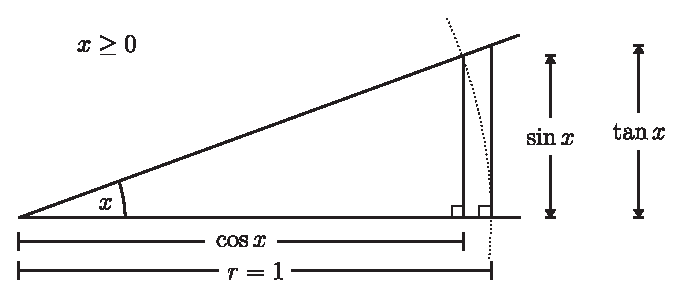
\includegraphics{skript/grafiken/vergleichkreissektor}
\end{center}
\begin{itemize}
    \item Aus der Grafik sieht man:
    $$ \underbrace{\frac{\cos x \cdot \sin x}{2}}_{\text{kleines Dreieck}} \leq \frac{x \cdot \pi}{2 \pi} \leq \underbrace{\frac{1 \cdot \tan x}{2}}_{\text{gro�es Dreieck}} $$
    Daraus folgt:
    $$ \cos x \leq \frac{x}{\sin x} \leq \frac{1}{\cos x} $$
    Nun kann den Limes f�r die beiden �u�eren Werte bestimmen:
    $$ \lim_{x \to 0+} \cos x = 1 = \lim_{x \to 0+} \frac{1}{\cos x} $$
    Damit folgt aus dem Vergleichskriterium:
    $$ \lim_{x \to 0-} \frac{x}{\sin x} = \lim_{x \to 0+} \frac{-x}{\sin (-x)} = \lim_{x \to 0+} \frac{x}{\sin x} = 1 $$
    Nun muss nur noch der Kehrwert betrachtet werden:
    $$ \lim_{x \to 0} \frac{\sin x}{x} = \frac{1}{\underset{x \to 0}{\lim} \frac{x}{\sin x}} = 1 $$
\end{itemize}
\pagebreak

%%%%%%%%%%%%%%%%%%%%%%%%%%%%%%%%%%%%%%%%%%%%%%%%%%%%%%%%%%%%%%%%%%%%%%%%%%%%%%%
\subsection{Stetigkeit}\index{Stetigkeit}
\textbf{Definition:\;} Es sei $I \subseteq \real$ ein Intervall und $f : I \rightarrow \real$ eine Funktion. \par \abstand
Die Funktion $f$ hei�t \emph{stetig} in $x_0 \in I$, wenn
$$ \lim_{x \to x_0} f(x) = f(x_0) $$
(wenn $x_0$ Rand von $I$, dann nur einseitiger Limes) \par \abstand

\textbf{Satz:\;} $f$ ist stetig in $x_0$ genau dann, wenn
$$ \forall \varepsilon > 0 \platz \exists \delta > 0 \platz \forall x \in I \platz (|x-x_0| < \delta \Rightarrow |f(x)-f(x_0)| < \varepsilon) $$

\textbf{Beweis ($\Leftarrow$):}
\begin{itemize}
    \item Zu zeigen ist: F�r jede Folge $(a_n)_{n \in \nat} \rightarrow x_0$ ist $\underset{n \to \infty}{\lim} f(a_n) = f(x_0)$.
    \item Das hei�t: $\forall \varepsilon > 0 \platz \exists n_0 \platz \forall n \geq n_0 \platz |f(a_n) - f(x_0)| < \varepsilon$.
    \item Man betrachtet $\delta > 0$ f�r das gegebene $\varepsilon$, da f�r $\underset{n \to \infty}{\lim} a_n = x_0$
    $$ \exists n_0 \platz \forall n \geq n_0 \platz |a_n - x_0| < \delta $$
    \item Behauptung:\; Dieses $n_0$ ist das gesuchte $n_0$.
    \item Sei $n \geq n_0$, dann gilt
    $$ |a_n - x_0| < \delta $$
    und nach Voraussetzung
    $$ |f(a_n) - f(x_0)| < \varepsilon $$
\end{itemize}
\pagebreak

\textbf{Beweis (indirekt, $\Rightarrow$):} Angenommen
$$ \exists \varepsilon > 0 \platz \forall \delta > 0 \platz \exists x \in I \platz (|x-x_0| < \delta \text{ und } |f(x) - f(x_0)|\geq \varepsilon) $$
dann konstruiert man eine Folge $(a_n)_{n \in \natpos}$, so dass
$$ \lim_{n \to \infty} a_n = x_0 \platz \text{aber} \platz \lim_{n \to \infty} f(a_n) \neq f(x_0) $$
\begin{eqnarray*}
    a_1 &:& \text{Setze } \delta = 1 \platz \exists \underset{\uparrow \atop a_1}{x} \in I \platz (|x - x_0| < \delta \text{ und } |f(x) - f(x_0)| \geq \varepsilon) \\
    a_n &:& \text{Setze } \delta = \frac{1}{n} \platz \exists \underset{\uparrow \atop a_n}{x} \in I \platz (|x - x_0| < \delta \text{ und } |f(x) - f(x_0)| \geq \varepsilon) \\
\end{eqnarray*}
Damit ist $\underset{n \to x_0}{\lim} a_n = x_0$ (da $|a_n - x_0| < \frac{1}{n}$), aber $|f(a_n) - f(x_0)| \geq \varepsilon$ f�r alle $n \in \nat$. \par \abstand
Daraus folgt: $f$ nicht stetig in $x_0$. \par \abstand \abstand

\textbf{Bemerkung:\;} Ist $f$ in $x_0$ nicht definiert, aber $\lim_{x \to x_0} f(x) \in \real$ existiert, dann kann man die Definition von $f$ auf $x_0$ erweitern durch $f(x_0) := \lim_{x \to x_0} f(x)$ ($f$ ist dann stetig in $x_0$). \par \abstand \abstand

\textbf{Beispiele:}
\begin{enumerate}
    \willbuch
    \item Rationale Funktionen schon per Definition stetig
    $$ f(x) = \frac{x^2 - 1}{x - 1} = \frac{(x-1) \cdot (x+1)}{x-1} = x+1 $$
    Damit ist $f(1) = 2$.
    \item $g(x) = \frac{\sin x}{x}$ ist auf $\real \backslash \{ 0 \}$ definiert.
    $$ g(0) := 1 $$
    \item $h(x) = \frac{\sqrt{x^2+1} - 1}{x^2}$ ist auf $\real \backslash \{ 0 \}$ definiert.
    $$ \lim_{x \to 0} \frac{\sqrt{x^2+1} - 1}{x^2} = \frac{1}{2} $$
    $$ h(0) := \frac{1}{2} $$
\end{enumerate}
\pagebreak

\textbf{Satz:\;} Sind $f$ und $g$ stetig auf $I$, dann sind auch
\begin{itemize}
    \item $f + g$, $f - g$ und $f \cdot g$ stetig auf $I$
    \item $\frac{f}{g}$ stetig in allen $x_0$, f�r die $g(x_0) \neq 0$
\end{itemize} \abstand

\textbf{Satz:\;} Wenn
\begin{itemize}
    \item die Funktion $f : I \rightarrow \real$ stetig auf $I$ ist,
    \item die Funktion $g : D \rightarrow \real$ stetig auf $D$ ist und
    \item das Bild $g(D) \subseteq I$ ist
\end{itemize}
dann ist $h(x) := f(g(x))$ stetig auf $D$. \par \abstand \abstand

\textbf{Folgerungen:}
\begin{itemize}
    \item Polynome sind auf $\real$ stetig.
    \item Rationale Funktionen $\frac{p(x)}{q(x)}$ mit $\text{ggT}(p(x), q(x)) = 1$ sind stetig in allen $x \in \real$ mit $q(x) \neq 0$.
\end{itemize} \abstand

\textbf{Satz:\;} F�r jede auf einem \emph{abgeschlossenen} Intervall $[a, b]$ stetige Funktion $f$ gilt:
\begin{itemize}
    \item Schrankensatz:
    $$ \exists K \in \real \platz \forall x \in [a, b] \platz |f(x)| < K $$
    \item Satz vom Minimum und Maximum:
    $$ \exists x_0, x_1 \in [a, b] \platz \forall x \in [a, b] \platz f(x_0) \leq f(x) \leq f(x_1)$$
    \item Zwischenwertsatz:
    $$ \forall c \platz f(x_0) \leq c \leq f(x_1) \platz \exists x \in [a, b] \platz f(x) = c $$
    \item Gleichm��ige Stetigkeit:
    $$ \forall \varepsilon > 0 \platz \exists \delta > 0 \platz \forall x, x' \in [a, b] \platz (|x - x'| < \delta \Rightarrow |f(x) - f(x')| < \varepsilon ) $$
\end{itemize}
\pagebreak

%%%%%%%%%%%%%%%%%%%%%%%%%%%%%%%%%%%%%%%%%%%%%%%%%%%%%%%%%%%%%%%%%%%%%%%%%%%%%%%
% Asymptotische Schranken (O-Notation)
%%%%%%%%%%%%%%%%%%%%%%%%%%%%%%%%%%%%%%%%%%%%%%%%%%%%%%%%%%%%%%%%%%%%%%%%%%%%%%%
\section{Asymptotische Schranken ($\bigO$-Notation)}
%%%%%%%%%%%%%%%%%%%%%%%%%%%%%%%%%%%%%%%%%%%%%%%%%%%%%%%%%%%%%%%%%%%%%%%%%%%%%%%
\subsection{Laufzeit}
\textbf{Anwendungen:\;} Laufzeitanalyse von Algorithmen \par \abstand

\textbf{Definition:\;} Die \wichtig{Laufzeit} $T(n)$ eines Algorithmus ist die maximale Anzahl der Schritte bei Eingaben der L�nge $n$. \par \abstand

\textbf{Beispiele:\;} $c_i$ ist eine Konstante, die modell- und implementierungsabh�ngig ist:
\begin{itemize}
    \item Bin�rsuche: \par
    $T_1(n) = c_1 \lceil \log_2 n \rceil$ \par
    \item Quicksort: \par
    $T_2(n) = c_2 \cdot n^2$
    \item Mergesort: \par
    $T_3(n) = c_3 \cdot n \cdot \lceil \log_2 n \rceil$
\end{itemize}

\textbf{Vergleich:\;} $T_2 = 3n^2$ und $T_3 = 100 \cdot n \cdot \log_2 n$
\begin{center}
    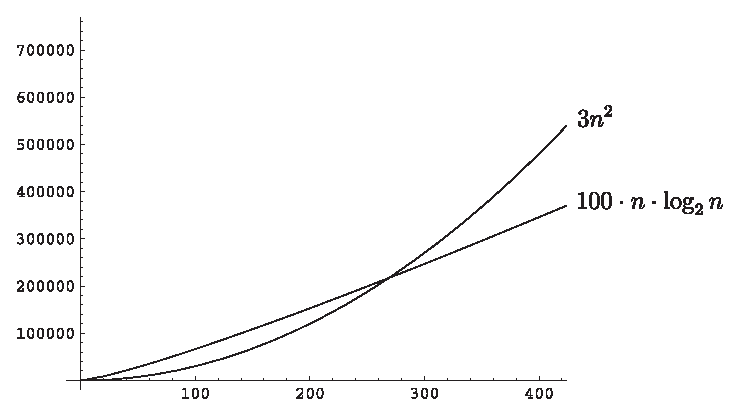
\includegraphics{skript/grafiken/onotation}
\end{center}
$$ \begin{array}{c|c|c|c|c}
  n & 3n^2 & \text{Zeit in $s$ bei 1 GHz} & 100n \cdot \lceil \log_2 n \rceil & \text{Zeit in $s$ bei 1 GHz} \\ \hline
  2 & 12 & 0,012 \text{ $\mu$s} & 200 & 0,2 \text{ $\mu$s} \\
  4 & 48 & 0,048 \text{ $\mu$s} & 800 & 0,8 \text{ $\mu$s} \\
  10^3 & 3 \cdot 10^6 & 3 \text{ ms} & \approx 10^6 & 1 \text{ ms} \\
  10^6 & 3 \cdot 10^{12} & 3000 s \approx 0,833 \text{ h} & \approx 2 \cdot 10^9 & 2 \text{ s} \\
  10^9 & 3 \cdot 10^{18} & 3 \cdot 10^9 \text{ s} \approx 100 \text{ Jahre} & \approx 3 \cdot 10^{12} & 3000 \text{ s} \approx 0,833 \text{ h}
\end{array} $$
\pagebreak

%%%%%%%%%%%%%%%%%%%%%%%%%%%%%%%%%%%%%%%%%%%%%%%%%%%%%%%%%%%%%%%%%%%%%%%%%%%%%%%
\subsection{Asymptotische Schranken}
\textbf{Definition:\;} $g(n)$ ist \wichtig{asymptotische obere Schranke} von $f(n)$, falls
\begin{itemize}
    \item eine Konstante $c > 0$  und
    \item ein $n_0 \in \nat$
\end{itemize}
existieren, so dass f�r alle $n \geq n_0$ gilt:
$$ f(n) \leq c \cdot g(n) $$
Schreibweise:
$$ f(n) = \bigO(g(n)) $$
\abstand

\textbf{Definition:\;} Seien $f$ und $g$ Funktionen $\nat \rightarrow \realpos$.
\begin{itemize}
    \item Obere Schranke:
    $$ \bigO(g(n)) = \{ f(n) \platz | \platz \exists c > 0 \platz \exists n_0 \platz \forall n \geq n_0 \platz f(n) \leq c \cdot g(n) \} $$
    \item Untere Schranke:
    $$ \Omega(g(n)) = \{ f(n) \platz | \platz \exists c > 0 \platz \exists n_0 \platz \forall n \geq n_0 \platz c \cdot g(n) \leq f(n) \} $$
    \item Wachstum
    $$ \Theta(g(n)) = \bigO(g(n) \cap \Omega(g(n))) $$
    \item Starke obere Schranke:
    $$ o(g(n)) = \{ f(n) \platz | \platz \forall c > 0 \platz \exists n_0 \platz \forall n \geq n_0 \platz f(n) \leq c \cdot g(n) \} $$
    \item Starke untere Schranke:
    $$ \omega(g(n)) = \{ f(n) \platz | \platz \forall c > 0 \platz \exists n_0 \platz \forall n \geq n_0 \platz c \cdot g(n) \leq f(n) \} $$
\end{itemize}

\textbf{Achtung:\;} $f(n) = \bigO(g(n))$ usw. hei�t eigentlich $f(n) \in O(g(n))$. \par \abstand
\pagebreak

\textbf{Lemma:}
\begin{eqnarray*}
  f(n) = \bigO(g(n)) & \Leftrightarrow & \left( \frac{f(n)}{g(n)} \right)_{n \in \nat} \text{ ist beschr�nkt} \\ \\
                     & \Leftrightarrow & g(n) = \Omega(f(n)) \\ \\ \\
  f(n) = o(g(n)) & \Leftrightarrow & \lim_{n \to \infty} \frac{f(n)}{g(n)} = 0 \\ \\
                 & \Leftrightarrow & g(n) = \omega(f(n))
\end{eqnarray*}

%%%%%%%%%%%%%%%%%%%%%%%%%%%%%%%%%%%%%%%%%%%%%%%%%%%%%%%%%%%%%%%%%%%%%%%%%%%%%%%
\subsection{Beispiele f�r Laufzeiten}
Funktionen, die bei Laufzeitabsch�tzung eine wichtige Rolle spielen:
\begin{itemize}
    \item $n$: jede Eingabestelle sehen
    \item $\log_2 n$: Teile-und-Herrsche-Prinzip
    \item $\sqrt{n}$: Anwendung von Seperatoren in planaren Graphen
    \item $2^n$: Untersuchung aller Teilmengen (Brute force)
    \item $n!$: Untersuchung aller Permutationen
\end{itemize}
\begin{itemize}
    \item Summen: Hintereinander-Ausf�hrung
    \item Produkte: geschachtelte Schleifen
\end{itemize}

Beispiel eines komplexen Ausdrucks:
\begin{itemize}
    \item $2^{\sqrt{n} \cdot \log_2 n}$: Faktorisierung $n$-stelliger Zahlen
\end{itemize}
\pagebreak

%%%%%%%%%%%%%%%%%%%%%%%%%%%%%%%%%%%%%%%%%%%%%%%%%%%%%%%%%%%%%%%%%%%%%%%%%%%%%%%
\subsection{Die wichtigsten Werkzeuge}
\textbf{Stirling-Formel:\;} Zur Absch�tzung von $n!$ kann folgende Formel benutzt werden:
$$ n! = \Omega \left( \sqrt{2 \pi n} \cdot \left( \frac{n}{e}^n \right) \right) $$
genauer:
$$ \sqrt{2 \pi n} \cdot \left( \frac{n}{e} \right)^n \platz \leq \platz n! \platz \leq \platz \sqrt{2 \pi n} \cdot \left( \frac{n}{e} \right)^{n + \frac{1}{12n}} $$

\textbf{Eigenschaften der Logarithmus-Funktion:} \par \abstand
Aufgrund der Definition des Logarithmus gilt:
$$ n = c^{\log_c n} $$

Anwendung:\; $T(n) = a^{\log_2 n}$
\begin{eqnarray*}
    a^{\log_2 n} &=& \left( 2^{\log_2 a} \right)^{\log_2 n} \\
                 &=& 2^{\log_2 a \cdot \log_2 n} \\
                 &=& \left( 2^{\log_2 n} \right)^{\log_2 n} \\
                 &=& n^{\log_2 a}
\end{eqnarray*}
Das hei�t: $T(n) = n^{\log_2 a}$ ein Polynom. \par \abstand

Umformungsregeln f�r Logarithmen:
\begin{itemize}
    \item $\frac{\log_a c}{\log_a b} = \log_b c$
    \item $\log_a b \cdot \log_b c = \frac{\ln b}{\ln a} \cdot \frac{\ln c}{\ln b} = \frac{\ln c}{\ln a} = \log_a c$
    \item $\log_a (f(n) \cdot g(n)) = \log_a f(n) + \log_a g(n)$
    \item $\log_a \frac{f(n)}{g(n)} = \log_a f(n) - \log_a g(n)$
    \item $\log_a b^c = c \cdot \log_a b$ \hfill (Folgerung: $\log_a n^k = \Theta(\log_a n)$)
\end{itemize}
\pagebreak

\textbf{Wachstum der Logarithmus-Funktion:} \par \abstand
Es gilt:
$$ f(n) = \bigO(g(n)) \platz \Rightarrow \platz \log_a (f(n)) = \bigO(\log_a (g(n))) $$
Beweis:
\begin{eqnarray*}
    f(n) &\leq& c \cdot g(n) \\ \\
    \Rightarrow \platz \log_a f(n) &\leq& \log_a (c \cdot g(n)) \\
                                   &=& \log_a c + \log_a g(n) \\
                                   &\leq& c' \cdot \log_a g(n) \platz (\text{mit } c' = \log_a (c + 1))
\end{eqnarray*}
Achtung:\; Die Regel gilt nicht f�r die starte obere Schranke!
$$ f(n) = o(g(n)) \platz \nRightarrow \platz \log_a (f(n)) = o(\log_a (g(n))) $$
Beispiel:
\begin{eqnarray*}
    f(n) = \sqrt{n} & & g(n) = n \\ \\
    \lim_{n \to \infty} \frac{f(n)}{g(n)} &=& \lim_{n \to \infty} \frac{\sqrt{n}}{n} \\
                                          &=& \lim_{n \to \infty} \frac{1}{\sqrt{n}} = 0 \\
                                          &\Rightarrow& f(n) = o(g(n)) \\ \\
    \lim_{n \to \infty} \frac{\log_a f(n)}{\log_a g(n)} &=& \lim_{n \to \infty} \frac{\log_a \sqrt{n}}{\log_a n} \\
                                                        &=& \lim_{n \to \infty} \frac{\frac{1}{2} \log_a n}{\log_a n} \\
                                                        &=& \lim_{n \to \infty} \frac{1}{2} = \frac{1}{2} \\
                                                        &\nRightarrow& \neg (\log_a f(n) = o(\log_a g(n)))
\end{eqnarray*}
\pagebreak

\textbf{Grundlagen f�r das Wachstum von Standardfunktionen:} \par \abstand
Seien $a, b \in \realpos$, dann gilt:
\begin{itemize}
    \item Wenn $a < b$, dann gilt
    $$ n^a = o(n^b) $$
    Beweis:
    $$ \underset{n \to \infty}{\lim} \frac{n^a}{n^b} = \underset{n \to \infty}{\lim} n^{a-b} = \underset{n \to \infty}{\lim} \frac{1}{n^{b-a}} = 0 $$
    \item Es gilt (auch wenn $b$ sehr gro� und $a$ sehr klein):
    $$ (\log_2 n)^b = o(n^a) $$
    \item Es gilt (auch wenn $b$ sehr gro� und $a$ sehr klein):
    $$ n^b = o(2^{a \cdot n}) $$
\end{itemize}

\pagebreak

%%%%%%%%%%%%%%%%%%%%%%%%%%%%%%%%%%%%%%%%%%%%%%%%%%%%%%%%%%%%%%%%%%%%%%%%%%%%%%%
%%%%%%%%%%%%%%%%%%%%%%%%%%%%%%%%%%%%%%%%%%%%%%%%%%%%%%%%%%%%%%%%%%%%%%%%%%%%%%%
% ab hier nicht korriegiert (reine Mitschrift, ohne Durchsicht) -->
%%%%%%%%%%%%%%%%%%%%%%%%%%%%%%%%%%%%%%%%%%%%%%%%%%%%%%%%%%%%%%%%%%%%%%%%%%%%%%%
%%%%%%%%%%%%%%%%%%%%%%%%%%%%%%%%%%%%%%%%%%%%%%%%%%%%%%%%%%%%%%%%%%%%%%%%%%%%%%%

%%%%%%%%%%%%%%%%%%%%%%%%%%%%%%%%%%%%%%%%%%%%%%%%%%%%%%%%%%%%%%%%%%%%%%%%%%%%%%%
% Polynominterpolation und Nullstellenbestimmung
%%%%%%%%%%%%%%%%%%%%%%%%%%%%%%%%%%%%%%%%%%%%%%%%%%%%%%%%%%%%%%%%%%%%%%%%%%%%%%%
\section{Polynominterpolation und Nullstellenbestimmung}
\textbf{Aufgabe:\;} Gegeben sind $n + 1$ Messpunkte $(x_0, y_0), (x_1, y_1), \ldots (x_n, y_n)$, wobei alle $x$-Werte verschieden sind. Gesucht wird ein Polynom $p(x)$ vom Grad $n$, so dass $p(x_i) = y_i$ f�r $i = 0 \ldots n$. \par \abstand
\textbf{Satz:\;} Zu $n+1$ St�tzpunkten $(x_0, y_0), (x_1, y_1), \ldots (x_n, y_n)$ mit $x_i \neq x_j$ gibt es \emph{genau} ein Polynom $p(x)$ vom Grad $\leq n$ mit $p(x_i) = y_i$ f�r $i = 0 \ldots n$. \par \abstand
\textbf{Beweis:}
\begin{enumerate}
    \item Existenz eines Polynoms $p(x)$ (Lagrange-Polynom): \par \abstand
    Es sei $0 \leq i \leq n$.
\end{enumerate}
\begin{eqnarray*}
  &\vdots& \\
  &\vdots& \\
  &\vdots& \\
  &\text{Vorlesung vom 18.6.2002 (fehlt)}& \\
  &\vdots& \\
  &\vdots& \\
  &\vdots&
\end{eqnarray*}
\pagebreak

\begin{eqnarray*}
  &\vdots& \\
  &\vdots& \\
  &\vdots& \\
  &\text{Vorlesung vom 20.6.2002 (fehlt)}& \\
  &\vdots& \\
  &\vdots& \\
  &\vdots&
\end{eqnarray*}

%%%%%%%%%%%%%%%%%%%%%%%%%%%%%%%%%%%%%%%%%%%%%%%%%%%%%%%%%%%%%%%%%%%%%%%%%%%%%%%
%%%%%%%%%%%%%%%%%%%%%%%%%%%%%%%%%%%%%%%%%%%%%%%%%%%%%%%%%%%%%%%%%%%%%%%%%%%%%%%
% nicht korriegiert (reine Mitschrift, ohne Durchsicht) -->
%%%%%%%%%%%%%%%%%%%%%%%%%%%%%%%%%%%%%%%%%%%%%%%%%%%%%%%%%%%%%%%%%%%%%%%%%%%%%%%
%%%%%%%%%%%%%%%%%%%%%%%%%%%%%%%%%%%%%%%%%%%%%%%%%%%%%%%%%%%%%%%%%%%%%%%%%%%%%%%

\chapter{Differentation}

%%%%%%%%%%%%%%%%%%%%%%%%%%%%%%%%%%%%%%%%%%%%%%%%%%%%%%%%%%%%%%%%%%%%%%%%%%%%%%%
% Ableitung einer differenzierbaren Funktion
%%%%%%%%%%%%%%%%%%%%%%%%%%%%%%%%%%%%%%%%%%%%%%%%%%%%%%%%%%%%%%%%%%%%%%%%%%%%%%%
\section{Ableitung einer differenzierbaren Funktion}
%%%%%%%%%%%%%%%%%%%%%%%%%%%%%%%%%%%%%%%%%%%%%%%%%%%%%%%%%%%%%%%%%%%%%%%%%%%%%%%
\begin{eqnarray*}
  &\vdots& \\
  &\vdots& \\
  &\vdots& \\
  &\text{Vorlesung vom 20.6.2002 (fehlt)}& \\
  &\vdots& \\
  &\vdots& \\
  &\vdots&
\end{eqnarray*}
\pagebreak

\begin{eqnarray*}
  &\vdots& \\
  &\vdots& \\
  &\vdots& \\
  &\text{Vorlesung vom 25.6.2002 (fehlt)}& \\
  &\vdots& \\
  &\vdots& \\
  &\vdots&
\end{eqnarray*}
\pagebreak

\textbf{Mittelwertsatz:\;} $f : [a b] \rightarrow \real$ (differentierbar)
$$ \exists x_0 \in (a, b) \platz f'(x_0) = \frac{f(b) - f(a)}{b-a} $$
\textbf{Folgerung 1:\;} $f : I \rightarrow \real$
\begin{eqnarray*}
    \text{$f'(x) > 0$ auf I} &\Rightarrow& \text{$f$ ist streng monoton wachsend} \\
    \text{$f'(x) < 0$ auf I} &\Rightarrow& \text{$f$ ist streng monoton fallend} \\
    \text{$f'(x) \geq 0$ auf I} &\Rightarrow& \text{$f$ ist monoton wachsend} \\
    \text{$f'(x) \leq 0$ auf I} &\Rightarrow& \text{$f$ ist monoton wachsend} \\
    \text{$f'(x) = 0$ auf I} &\Rightarrow& \text{$f$ ist konstant}
\end{eqnarray*}

\textbf{Beweis (indirekt):\;} Folgt aus dem Mittelwertsatz \par \abstand

\textbf{Folgerung 2:\;} $f, g : I \rightarrow \real$ und $f'(x) = g'(x)$ auf I
$$ f(x) = g(x) + c $$
\textbf{Beweis:}
$$ [ f(x) - g(x) ]' = f'(x) - g'(x) = 0 \platz \rightarrow \platz f(x) - g(x) \text{ ist konstant} $$

\subsection{Station�re Punkte}
\textbf{Definition:\;} Nullstellen der ersten Ableitung $f'(x)$ werden \wichtig{station�re Punkte} von $f$ genannt. \par \abstand

Welche station�ren Punkte sind lokale Extrema?
\begin{itemize}
    \item Notwendig: $f'(x) = 0$
    \item Hinrichend f�r Maximum: $f$ ist streng monoton wachsend links von $x$ und streng monoton fallend rechts von $x$, d.h.
    \begin{itemize}
        \item $f' > 0$ links von $x$
        \item $f' < 0$ rechts von $x$
    \end{itemize}
    \begin{center}
        GRAFIK: Graph mit Maximum und Ableitung
    \end{center}
    also: $f''(x) < 0$
    \item Hinreichend f�r Minimum: entsprechend $f''(x) > 0$
\end{itemize}

Die zweite Ableitung beschreibt die Kr�mmung der Funktionskurve von $f$.
\begin{center}
    GRAFIK
\end{center}
\begin{itemize}
    \item $f''(x) > 0$: Kurve ist linksgekr�mmt (konvex von unten)
    \item $f''(x) < 0$: Kurve ist rechtsgekr�mmt (konvex von oben)
\end{itemize}

\textbf{Wendepunkt:\;} Ein Wendepunkt ist ein Punkt, in dem Linkskr�mmung in Rechtskr�mmung �bergeht (oder umgekehrt).
\begin{itemize}
    \item notwendige Bedingung: $f''(x) = 0$
    \item hinreichende Bedingung: $f'''(x) \neq 0$
\end{itemize}

\textbf{Satz (Verallgemeinerter Mittelwertsatz):\;} $f, g : [a, b] \rightarrow \real$ (differenzierbar in $(a, b)$, stetig auf $[a, b]$ und $g'(x) \neq 0$ in $(a, b)$). \par \abstand
Es existiert ein $x_0 \in (a, b)$ mit
$$ \frac{f(b) - f(a)}{g(b) - g(a)} = \frac{f'(x_0)}{g'(x_0)} $$
\textbf{Beweis:\;} $g(a) \neq g(b)$ wegen $g'(x) \neq 0$ (da entweder streng monoton wachsend oder fallend)
$$ F(x) := f(x) - \frac{f(b) - f(a)}{g(b) - g(b)} \cdot g(x) $$
Mittelwertsatz f�r $F$:
$$ F(a) = \frac{f(a) \cdot g(b) - f(b) \cdot g(a)}{g(b) - g(a)} = F(b) $$
$$ \exists x_0 \platz F'(x_0) = 0$$
Daraus folgt:
$$ 0 = f'(x_0) - \frac{f(b) - f(a)}{g(b) - g(a)} \cdot g'(x) $$
$$ \frac{x_0}{g'(x_0)} = \frac{f(b) - f(a)}{g(b) - g(a)} $$

\textbf{Satz (Regel von Bernoulli-L'Hospital):\;} $f, g: (a, b) \rightarrow \real$ \par \abstand
Voraussetungen:
\begin{itemize}
    \item differenzierbar auf $(a, b)$
    \item $g'(x) \neq 0$ auf $(a, b)$
    \item $f(x) \underset{x \to b-}{\longrightarrow} 0$ und $g(x) \underset{x \to b-}{\longrightarrow} 0$ oder \par
    $f(x) \underset{x \to b-}{\longrightarrow} \infty$ und $g(x) \underset{x \to b-}{\longrightarrow} \infty$
    \item $\underset{x \to b-}{\lim} \frac{f'(x)}{g'(x)} \in \real \cup \{ \pm \infty \}$
\end{itemize}
Dann ist:
$$ \lim_{x \to b-} \frac{f(x)}{g(x)} = f $$
\textbf{Beweis:\;} Nur $f(x), g(x) \underset{x \to b-}{\longrightarrow} 0$ \par \abstand
\begin{itemize}
    \item Setzen $f(b) = g(b) = 0$ (stetige Erweiterung)
    \item F�r jedes $x \in (a, b)$ betrachten wie verallgemeinerten Mittelwertsatz auf $[x, b]$.
    $$ \exists x_0 \in (x, b) \platz \frac{f'(x_0)}{g'(x_0)} = \frac{f(b) - f(x)}{g(b) - g(x)} = \frac{f(x)}{g(x)} $$
    \item Daraus folgt:
    $$ x \to b- \platz \Rightarrow \platz x_0 \to b- \platz \rightarrow \platz \lim_{x \to b-} \frac{f'(x_0)}{g'(x_0)} = \lim_{x \to b-} \frac{f(x)}{g(x)} $$
\end{itemize}

\textbf{Anwenundung oft nach vorherigen Umformungen:\;}
\begin{eqnarray*}
  \lim_{x \to 0+} \left( \frac{1}{x} - \frac{1}{1 - \cos x} \right) &=& - \infty \\
  \frac{1}{x} - \frac{1}{1 - \cos x} &=& \frac{\overbrace{1 - \cos x - x}^{f(x)}}{\underbrace{x \cdot (1 - \cos x)}_{g(x)}} \\ \\
  \frac{f'(x)}{g'(x)} &=& \frac{\sin x - 1}{(1 - \cos x) + x \cdot \sin x} \underset{x \to 0+}{\longrightarrow} = - \infty
\end{eqnarray*}

%%%%%%%%%%%%%%%%%%%%%%%%%%%%%%%%%%%%%%%%%%%%%%%%%%%%%%%%%%%%%%%%%%%%%%%%%%%%%%%
\section{Umkehrfunktion}
$f : I \rightarrow \real, D \subseteq I$ \par \abstand
$f$ ist umkehrbar auf $D$, falls die eingeschr�nkte Funktion
$$ f |_D : D \rightarrow f(D) = \text{Im}(f |_D)  $$
ist bijektiv. \par \abstand

\textbf{Beispiel:}
\begin{itemize}
    \item $f(x) = x^2$ ($I = \real$)
    \item $f |_{\realpos} : \realpos \rightarrow \realpos$ bijektiv
    \item Umkehrfunktion $f^{-1}(x) = \sqrt{x}$
    \item $x^2$ auch umkehrbar �ber $\real^-$: $f^{-1}(x) = - \sqrt{x}$
    \begin{center}
        GRAFIK: $x^2$ hat zu $\sqrt{x}$ eine Symmetrieachse, aber auch $- \sqrt{x}$
    \end{center}
\end{itemize}

\textbf{Satz:}
\begin{enumerate}
    \willbuch
    \item $f$ streng monoton auf $D$, daraus folgt $f$ umkehrbar auf $D$, d.h. $f$ differenzierbar auf $D$ und $f'(x) \neq 0$ auf $D$ $\Rightarrow$ $f$ umkehrbar auf $D$
    \item Die Graphen von $f$ und der Umkehrung $f^{-1}$ sind symmetrisch bez�glich derGeraden $y = x$.
    \item Ist $f : I \rightarrow \real$ �ber $D$ umkehrbar und differenzierbar, so ist auch die Umkehrfunktion $g : f(D) \rightarrow \real$ in allen $x \in f(D)$ differenzierbar und es gilt $g'(x) = \frac{1}{f'(g(x))}$.
\end{enumerate}

\textbf{Beweis c):}
\begin{align*}
    \frac{1}{f'(g(x))} &= \frac{1}{\underset{y \to g(x)}{\lim} \frac{f(y) - f(g(x))}{y - g(x)}} \\
    \intertext{$g$ stetig, $x' \to x$, dann $g(x') \to g(x)$}
                       &= \frac{1}{\underset{x' \to x}{\lim} \frac{f(g(x')) - f(g(x))}{g(x') - g(x)}} \\
    \intertext{$g$ ist Umkehrfunktion von $f$, also $fg = \text{Id}$}
                       &= \frac{1}{\underset{x' \to x}{\lim} \frac{x' - x}{g(x') - g(x)}} \\
                       &= \underset{x' \to x}{\lim} \frac{g(x') - g(x)}{x' - x} \\
                       &= g'(x)
\end{align*}

\textbf{Beispiele:}
\begin{enumerate}
    \item $f(x) = x^3$ mit $f : \real \to \real$ \\
    $f'(x) = 3x^2 \geq 0$, $f$ ist streng monoton wachsend, $f$ ist umkehrbar
    \begin{eqnarray*}
        f^{-1}(x) &=& \sqrt[3]{x} \\
        \left( \sqrt[3]{x} \right)' &=& \frac{1}{3 \left( \sqrt[3]{x} \right)^2 } = \frac{1}{3} x^{-\frac{2}{3}}
    \end{eqnarray*}
    \item $f(x) = x^n$, $n$ gerade, $f$ ist umkehrbar �ber $\realpos$ oder \\
    $f(x) = x^n$, $n$ ungerade, $f$ ist umkehrbar �ber $\real$
    \begin{eqnarray*}
        \sqrt[n]{x} = x^{\frac{1}{n}} \\
        \left( \sqrt[n]{x} \right)' &=& \frac{1}{n \left( \sqrt[n]{x} \right)^{n-1} } = \frac{1}{n} \cdot x^{\frac{-n+1}{n}}
    \end{eqnarray*}
    rationale Potenzen: \\
    $f_{\alpha}(x) = x^{\alpha}$ mit $\alpha = \frac{m}{n} \in \rat$, $n > 0$
    $$ f_{\alpha}(x) = \left\{ \begin{array}{l@{\text{ falls }}l}
        \sqrt[n]{x} & m > 0 \\
        1 & m = 0 \\
        \frac{1}{\left( \sqrt[n]{x} \right)^{-m}} & m < 0
    \end{array} \right. $$
    Einheitlicher Definitionsbereich $\realpos$
    \begin{eqnarray*}
        f'_{\alpha}(x) &=& m \cdot \left( \sqrt[n]{x} \right)^{m-1} \cdot \frac{1}{n \cdot \left( \sqrt[n]{x} \right)^{n-1} } \\
                       &=& \frac{m}{n} \cdot \left( \sqrt[n]{x} \right)^{m-1-(n-1)} \\
                       &=& \frac{m}{n} \cdot \left( \sqrt[n]{x} \right)^{m-n} \\
                       &=& \frac{m}{n} \cdot x^{\frac{m-n}{n}} \\
                       &=& \alpha \cdot x^{\alpha - 1}
    \end{eqnarray*}
    \item Winkelfunktionen
    \begin{center}
        GRAFIK: $\sin : \real \to [-1, 1]$
    \end{center}
    $\sin : \real \to [-1, 1]$, umkehrbar auf $\left[ - \frac{\pi}{2}, \frac{\pi}{2} \right]$, da $\cos$ in diesem Bereich $\geq 0$, also $\sin$ monoton steigend \\
    Umkehrfunktion: $\arcsin : [-1, 1] \to [-\frac{\pi}{2}, \frac{\pi}{2} ] $ (0-ter Zweig von $\arcsin$) \\
    1. Zweig w�re z.B. die Umkehrung von $\sin$ auf $\left[ \frac{\pi}{2}, \frac{3 \pi}{2} \right]$ \par \abstand
    Ableitung:
    Aus $\arcsin x \in [-\frac{\pi}{2}, \frac{\pi}{2}]$ folgt $\cos(\arcsin x) \geq 0$ \\
    $\cos y = \sqrt{1 - \sin^2 y}$ f�r $y \in [-\frac{\pi}{2}, \frac{\pi}{2}]$, da $\cos$ in diesem $\geq 0$
    \begin{eqnarray*}
        (\arcsin x)' &=& \frac{1}{\cos(\arcsin x)} \\
                     &=& \frac{1}{\sqrt{1 - \sin^2 (\arcsin x)}} \\
                     &=& \frac{1}{\sqrt{1 - x^2}}
    \end{eqnarray*}
    $\cos : \real \to [-1, 1]$ umkehrbar auf $[0, \pi]$ \\
    $\arccos : [-1, 1] \to [0, \pi]$
    $$ (\arccos x)' = - \frac{1}{\sqrt{1 - x^2}} $$
    $\tan : \real \backslash \{ \frac{\pi}{2} + k \pi \} \to (- \infty, + \infty)$ \\
    umkehrbar auf $(-\frac{\pi}{2}, \frac{\pi}{2})$ \\
    $\arctan : \real \to (- \frac{\pi}{2}, \frac{\pi}{2})$
    \begin{eqnarray*}
        (\arctan' x)' &=& \frac{1}{\tan'(\arctan x)} \\
                      &=& \frac{1}{\frac{sin^2(\arctan x) + \cos^2(\arctan x)}{\cos^2(\arctan x)}} \\
                      &=& \frac{1}{\tan^2(\arctan x) + 1} \\
                      &=& \frac{1}{x^2 + 1}
    \end{eqnarray*}
    $\text{arccot } : \real \to (0, \pi)$
    $$ (\text{arccot } x)' = - \frac{1}{x^2 + 1} $$
    \item Exponentialfunktion:
    $$ \exp(x) = \underset{n \to \infty}{\lim} \left( 1 + \frac{x}{n} \right)^n = e^x $$
    Idee f�r Ableitung:
    \begin{eqnarray*}
        \frac{d}{dx} e^x &=& \frac{d}{dx} \overset{n \to \infty}{\lim} \left( 1 + \frac{1 + \frac{x}{n}}{} \right)^n \\
                         &\overset{?}{=}& \underset{n \to \infty}{\lim} \frac{d}{dx} \left( 1 + \frac{x}{n} \right)^n \\
                         &=& \underset{n \to \infty}{\lim} \left[ n \cdot \left( 1 + \frac{x}{n} \right)^{n-1} \cdot \frac{1}{n} \right] \\
                         &=& \frac{\underset{n \to \infty}{\lim} \left( 1 + \frac{x}{n} \right)^n}{\underset{n \to \infty}{\lim} \left( 1 + \frac{x}{n} \right)}
    \end{eqnarray*}
    genaue Gr�ndung mit Mittelwertsatz!
    Daraus folgt: $\exp'(x) = \exp(x)$ \\
    Aus $e^x > 0$ folgt, dass $\exp$ streng monoton wachsend ist \\
    $\exp$ ist umkehrbar �ber $\real$ \\
    Umkehrfunktion: $\ln : \realpos \to \real$
    $$ \ln' x = \frac{1}{\exp'(\ln x)} = \frac{1}{\exp(\ln x)} = \frac{1}{x} $$
\end{enumerate}

%%%%%%%%%%%%%%%%%%%%%%%%%%%%%%%%%%%%%%%%%%%%%%%%%%%%%%%%%%%%%%%%%%%%%%%%%%%%%%%
%%%%%%%%%%%%%%%%%%%%%%%%%%%%%%%%%%%%%%%%%%%%%%%%%%%%%%%%%%%%%%%%%%%%%%%%%%%%%%%
% nicht korriegiert (reine Mitschrift, ohne Durchsicht) -->
%%%%%%%%%%%%%%%%%%%%%%%%%%%%%%%%%%%%%%%%%%%%%%%%%%%%%%%%%%%%%%%%%%%%%%%%%%%%%%%
%%%%%%%%%%%%%%%%%%%%%%%%%%%%%%%%%%%%%%%%%%%%%%%%%%%%%%%%%%%%%%%%%%%%%%%%%%%%%%%

\chapter{Integration}

%%%%%%%%%%%%%%%%%%%%%%%%%%%%%%%%%%%%%%%%%%%%%%%%%%%%%%%%%%%%%%%%%%%%%%%%%%%%%%%
% Stammfunktionen
%%%%%%%%%%%%%%%%%%%%%%%%%%%%%%%%%%%%%%%%%%%%%%%%%%%%%%%%%%%%%%%%%%%%%%%%%%%%%%%
\section{Stammfunktionen}
%%%%%%%%%%%%%%%%%%%%%%%%%%%%%%%%%%%%%%%%%%%%%%%%%%%%%%%%%%%%%%%%%%%%%%%%%%%%%%%
\textbf{Definition:\;} Eine auf dem Intervall $I$ differenzierbare Funktion $F$ ist eine Stammfunktion der Funktion $f : I \to \real$, wnn $F'(x)= f(x)$ f�r alle $x \in I$. \par \abstand
Fakt 1: Sind $F_1$ und $F_2$ Stammfunktionen von $f$, dann gilt $F_1(x) = F_2(x) + c$ f�r alle $x \in I$ und ein $c \in \real$ (aus dem Mitterlwertsatz). \par \abstand

\textbf{Definition:\;} Die Menge aller Stammfunktionen von $f$ wird das unbestimmte Integral von $f$ genannt und mit $\int f(x) dx = F(x) + c$ bezeichnet.


% Indexverzeichnis
\printindex

\end{document}
